\documentclass[a4paper]{report}
\usepackage{graphicx}
\usepackage{booktabs}
\usepackage{pdfpages}
\DeclareGraphicsRule{.docx}{pdf}{.pdf}{`pandoc #1 -o \noexpand\OutputFile}

\title{Foreign Exchange Management System (FXMS)}
\author{
    Yazeed AlKhalaf \\
    Mohammed Bin Jebreen \\
    Nawaf AlAmer \\
    \textbf{Course:} SWE 301 - Requirements Engineering \\
    \textbf{Instructor:} Dr. Noureddine Abbadeni
}
\date{3 Mar, 2024}

\begin{document}

\maketitle

\newpage

\tableofcontents

\chapter{System Request (FXMS)}

\section{Project Sponsor}
Dr. Noureddine Abbadeni

\section{Business Need}
The need for a project like the Foreign Exchange Management System (FXMS) is crucial for businesses operating internationally for several reasons:
\begin{itemize}
    \item \textbf{Operating internationally:} Businesses engaged in importing and exporting goods and services will need a system like FXMS for currency conversion, enabling them to exchange their local currency for that of the country in which they wish to operate, thereby settling international transactions.
    \item \textbf{Managing cash flow:} Businesses operating overseas need to manage their cash across multiple currencies. FXMS will help them monitor and optimize their cash by converting currency at favorable rates and timings.
    \item \textbf{Softening the risk:} FXMS will provide businesses with tools to manage and mitigate the risks associated with fluctuations in currency prices. By using specific strategies, companies can lower the risk of exchange rate volatility and protect their profit margins.
\end{itemize}

\section{Business Requirements}
The functionality that the system should have includes:
\begin{itemize}
    \item Ability to manage clients and accounts (insert, update, delete).
    \item Ability to manage trades (insert, update, and delete trades). Any trader can enter new trades while updating and deleting existing trades require specific privileges.
    \item Ability to manage traders and coverage groups by assigning a trader to a coverage group, moving a trader from one coverage group to another.
    \item Ability to manage currencies and rates including daily updates of rates available in the market. The system is assumed to be connected with another system (such as Tadawul) which provides daily updates for exchange rates between all currencies.
    \item The system will integrate with two systems: FX trading database and FX coverage group database. These two systems are the main data sources for the system.
\end{itemize}

\section{Business Value}
The Foreign Exchange Management System (FXMS) is expected to deliver significant gains:
\begin{itemize}
    \item \textbf{Quicker and Better Decision Making:} Facilitated by the collection of multiple systems, enhancing competitive advantage in international markets.
    \item \textbf{Less Human Error:} The human factor is limited to tasks that require human interaction and not repetitive tasks that are error-prone.
    \item \textbf{More Money:} The efficient management of trades and currency conversions is expected to increase the organization's revenue.
    \item Headcount reduction by 10 traders per branch.
    \item 15\% increase in market share.
\end{itemize}

\section{Constraints}
\begin{itemize}
    \item The system should run on Windows 10.
    \item The system should be delivered by the end of the year 2028.
    \item Security and reliability must be considered during development.
\end{itemize}

\chapter{Feasibility Study}

Overall, the risk in this project compared to the gains can be considered manageable.

\section{Technical}

The technical team is confident they can build it since they built a similar system before, the knowldege they gained during that experience lowers the risk.

\begin{itemize}
    \item \textbf{Familiarity with application:} The team is familiar with building an FXMS.
    \item \textbf{Familiarity with technology:} Since the team members have a collective experience of over 50 years building complex software, we are confident they will be able to tackle the project.
    \item \textbf{Project Size:} Large project.
    \item \textbf{Compatibility:} The company wants a custom solution, so we will make sure it integrates well by analysing before we build anything and before we choose a platform.
\end{itemize}

The techincal team is confident they can build the system even though it is big. They have built a similar system before and they are familiar with the requirements and the technology.

\newpage

\section{Financial}

\subsection{Cost-Benefit Analysis}

The cashflow analysis below in Figure \ref{fig:cash-flow-analysis} is a condensed versin of the 4 years (monthly based) version of the cashflow analysis. It gives an idea on the way the project will behave financially.

\begin{figure}[h!]
    \centering
    \includegraphics[width=0.8\textwidth]{images/cash-flow-analysis.png}
    \caption{Cashflow Analysis of FXMS}
    \label{fig:cash-flow-analysis}
\end{figure}

\subsection{ROI and BEP}

We will move to the big numbers, the ROI and the BEP.

\begin{figure}[h!]
    \centering
    \includegraphics[width=0.8\textwidth]{images/roi-bep.png}
    \caption{ROI and BEP of FXMS}
    \label{fig:roi-and-bep}
\end{figure}

\subsection{Conclusion}

The project overall risk is medium. Although the team familiarity is high, the system's dependencies and huge footprint makes us consider the project as medium risk.

\chapter{Methodology}

Now we will evaluate the methodologies we can use to build the system. We will follow a three step approach to help us choose the right methodology. The three steps are:

\begin{enumerate}
    \item \textbf{Criteria:} We will list the criteria we will use to evaluate the methodologies and answer them according to our familiarity.
    \item \textbf{Evaluation:} We will evaluate the methodologies based on the criteria answers above. This will help us in choosing the right methodology.
    \item \textbf{Selection:} We will choose the methodology that fits the use case. It might not be a 100\% fit, it would be the most suitable one.
\end{enumerate}

\section{Criteria}

The criteria we will use to evaluate the methodologies are shown and answered in Table \ref{tab:criteria-answers}.

\begin{table}[htbp]
    \centering
    \caption{Criteria Answers for System Development Methodologies}
    \label{tab:criteria-answers}
    \begin{tabular}{@{}p{0.5\linewidth}cc@{}}
        \toprule
        Criteria                                         & Answer \\
        \midrule
        Are the requiremnts unclear?                     & Yes    \\
        Are we unfamiliar with the technology?           & No     \\
        Are the requirements complex?                    & Yes    \\
        Should the system be reliable?                   & Yes    \\
        Is time allocated for building the system short? & No     \\
        Do we have schedule visibility?                  & No     \\
        \bottomrule
    \end{tabular}
\end{table}

\section{Evaluation}

We will evaluate the methodologies based on the criteria answers above. The following table, \ref{tab:criteria-evaulation}, shows each criteria and the methodology that fits it based on our answer from the previous section in Table \ref{tab:criteria-answers}.

\begin{table}[htbp]
    \centering
    \caption{Criteria Evaluation for System Development Methodologies}
    \label{tab:criteria-evaulation}
    \begin{tabular}{@{}p{0.5\linewidth}cc@{}}
        \toprule
        Criteria                                 & Fit Methodology                  \\
        \midrule
        Requirements are clear                   & All                              \\
        Team is familiar with techonology        & All                              \\
        Requirments are complex                  & Throwaway Prototyping            \\
        System should be relable                 & V-Model \& Throwaway Prototyping \\
        Time allocated for building is not short & All                              \\
        We don't have schedule visibility        & All                              \\
        \bottomrule
    \end{tabular}
\end{table}

\section{Selection}

Based on the evaluation above, we will choose the methodology that fits the use case. The methodology that fits the use case is the "Throwaway Prototyping" methodology. This methodology fits the use case because the requirements are complex and the system should be reliable. And since other criterions are not a problem, we can choose this methodology.

\chapter{Project Workplan}

The project workplan is shown in Figure \ref{fig:wbs}. The project is divided into 7 main phases after the "Kick off meeting". The phases are:

\begin{itemize}
    \item \textbf{Requirements Gathering:} This phase will be done by Nawaf.
    \item \textbf{Business Case:} This phase will be done by Mohammed.
    \item \textbf{System Design:} This phase will be done by Yazeed.
    \item \textbf{Analysis:} This phase will be done by Nawaf.
    \item \textbf{Design:} This phase will be done by Mohammed.
    \item \textbf{Development:} This phase will be done by Yazeed.
    \item \textbf{Quality Assurance:} This phase will be done by Nawaf.
    \item \textbf{Testing:} This phase will be done by Yazeed.
\end{itemize}

\begin{figure}[h!]
    \centering
    \includegraphics[width=0.8\textwidth]{images/wbs.png}
    \caption{Workplan Breadown Structure (WBS) of FXMS}
    \label{fig:wbs}
\end{figure}

\chapter{Gathering/Elicitation Techniques}

\begin{itemize}
    \item \textbf{Type of information:} A mix between as-is (existing data sources) and to-be (our new system). The techniques that appeal are:
          \begin{itemize}
              \item Interviews
              \item Joint Application Design (JAD)
          \end{itemize}
    \item \textbf{Depth of information:} High depth of information is required since the system is complex and deals with financial information, we can't affoed losses because of aasumptions. Hence, the techniques that appeal are:
          \begin{itemize}
              \item Interviews
              \item Joint Application Design (JAD)
          \end{itemize}
    \item \textbf{Breadth of information:} Medium breadth of information is required. The techniques that appeal are:
          \begin{itemize}
              \item Joint Application Design (JAD)
          \end{itemize}
    \item \textbf{Integration of information:} We need to integrate data from different stakeholders, so high integration is required. The techniques that appeal are:
          \begin{itemize}
              \item Joint Application Design (JAD)
          \end{itemize}
    \item \textbf{User Involvement:} High involvement is required. The techniques that appeal are:
          \begin{itemize}
              \item Joint Application Design (JAD)
          \end{itemize}
    \item \textbf{Cost:} Since the time required to do the project is short, money shouldn't be a problem. All techniques are low to medium so all of the apply here.
\end{itemize}

Based on the facts stated below for each criterion, we have concluded that the most suitable techniques:

\begin{itemize}
    \item Interviews
    \item Joint Application Design (JAD)
\end{itemize}

\chapter{Requirements Analysis}

After carefully analysing the requirements there are some things concerning them and there are some contradictions as well as missing parts. Examples of this are in the Functional requirements (FR):

\begin{itemize}
    \item It was stated that the system will have the ability to manage clients and accounts which incudes inserting updating and deleting, but who has the privileges to this action?
          \begin{itemize}
              \item \textbf{Solution:} Assign the privileges to the admin.
          \end{itemize}
    \item It was stated that the system will have the ability to manage trades as well as inserting updating and deleting trades as well as entering new trades while updating and deleting existing trades which require specific privileges what are the privileges who has these privileges.
          \begin{itemize}
              \item \textbf{Solution:} Assign the privileges to the admin.
          \end{itemize}
    \item It was also stated that the system will have the ability to manage traders and coverage groups by assigning a trader to a coverage groups but the question is who will have the privileges to execute this actions?
          \begin{itemize}
              \item \textbf{Solution:} Assign the privileges to the admin.
          \end{itemize}
\end{itemize}


\chapter{List of Stakeholders}

Based on the information provided, the following stakeholders can be identified:
\begin{itemize}
    \item Traders
    \item Clients (Organizations and Companies)
    \item Coverage Groups
    \item Investment Bank (Business User/Sponsor)
\end{itemize}

\chapter{System Boundary}

We have identified the system boundary as shown in the figure below in Figure \ref{fig:system-boundary}. The system boundary includes both our new system and the two data courses we will be integrating with.

\begin{figure}[h!]
    \centering
    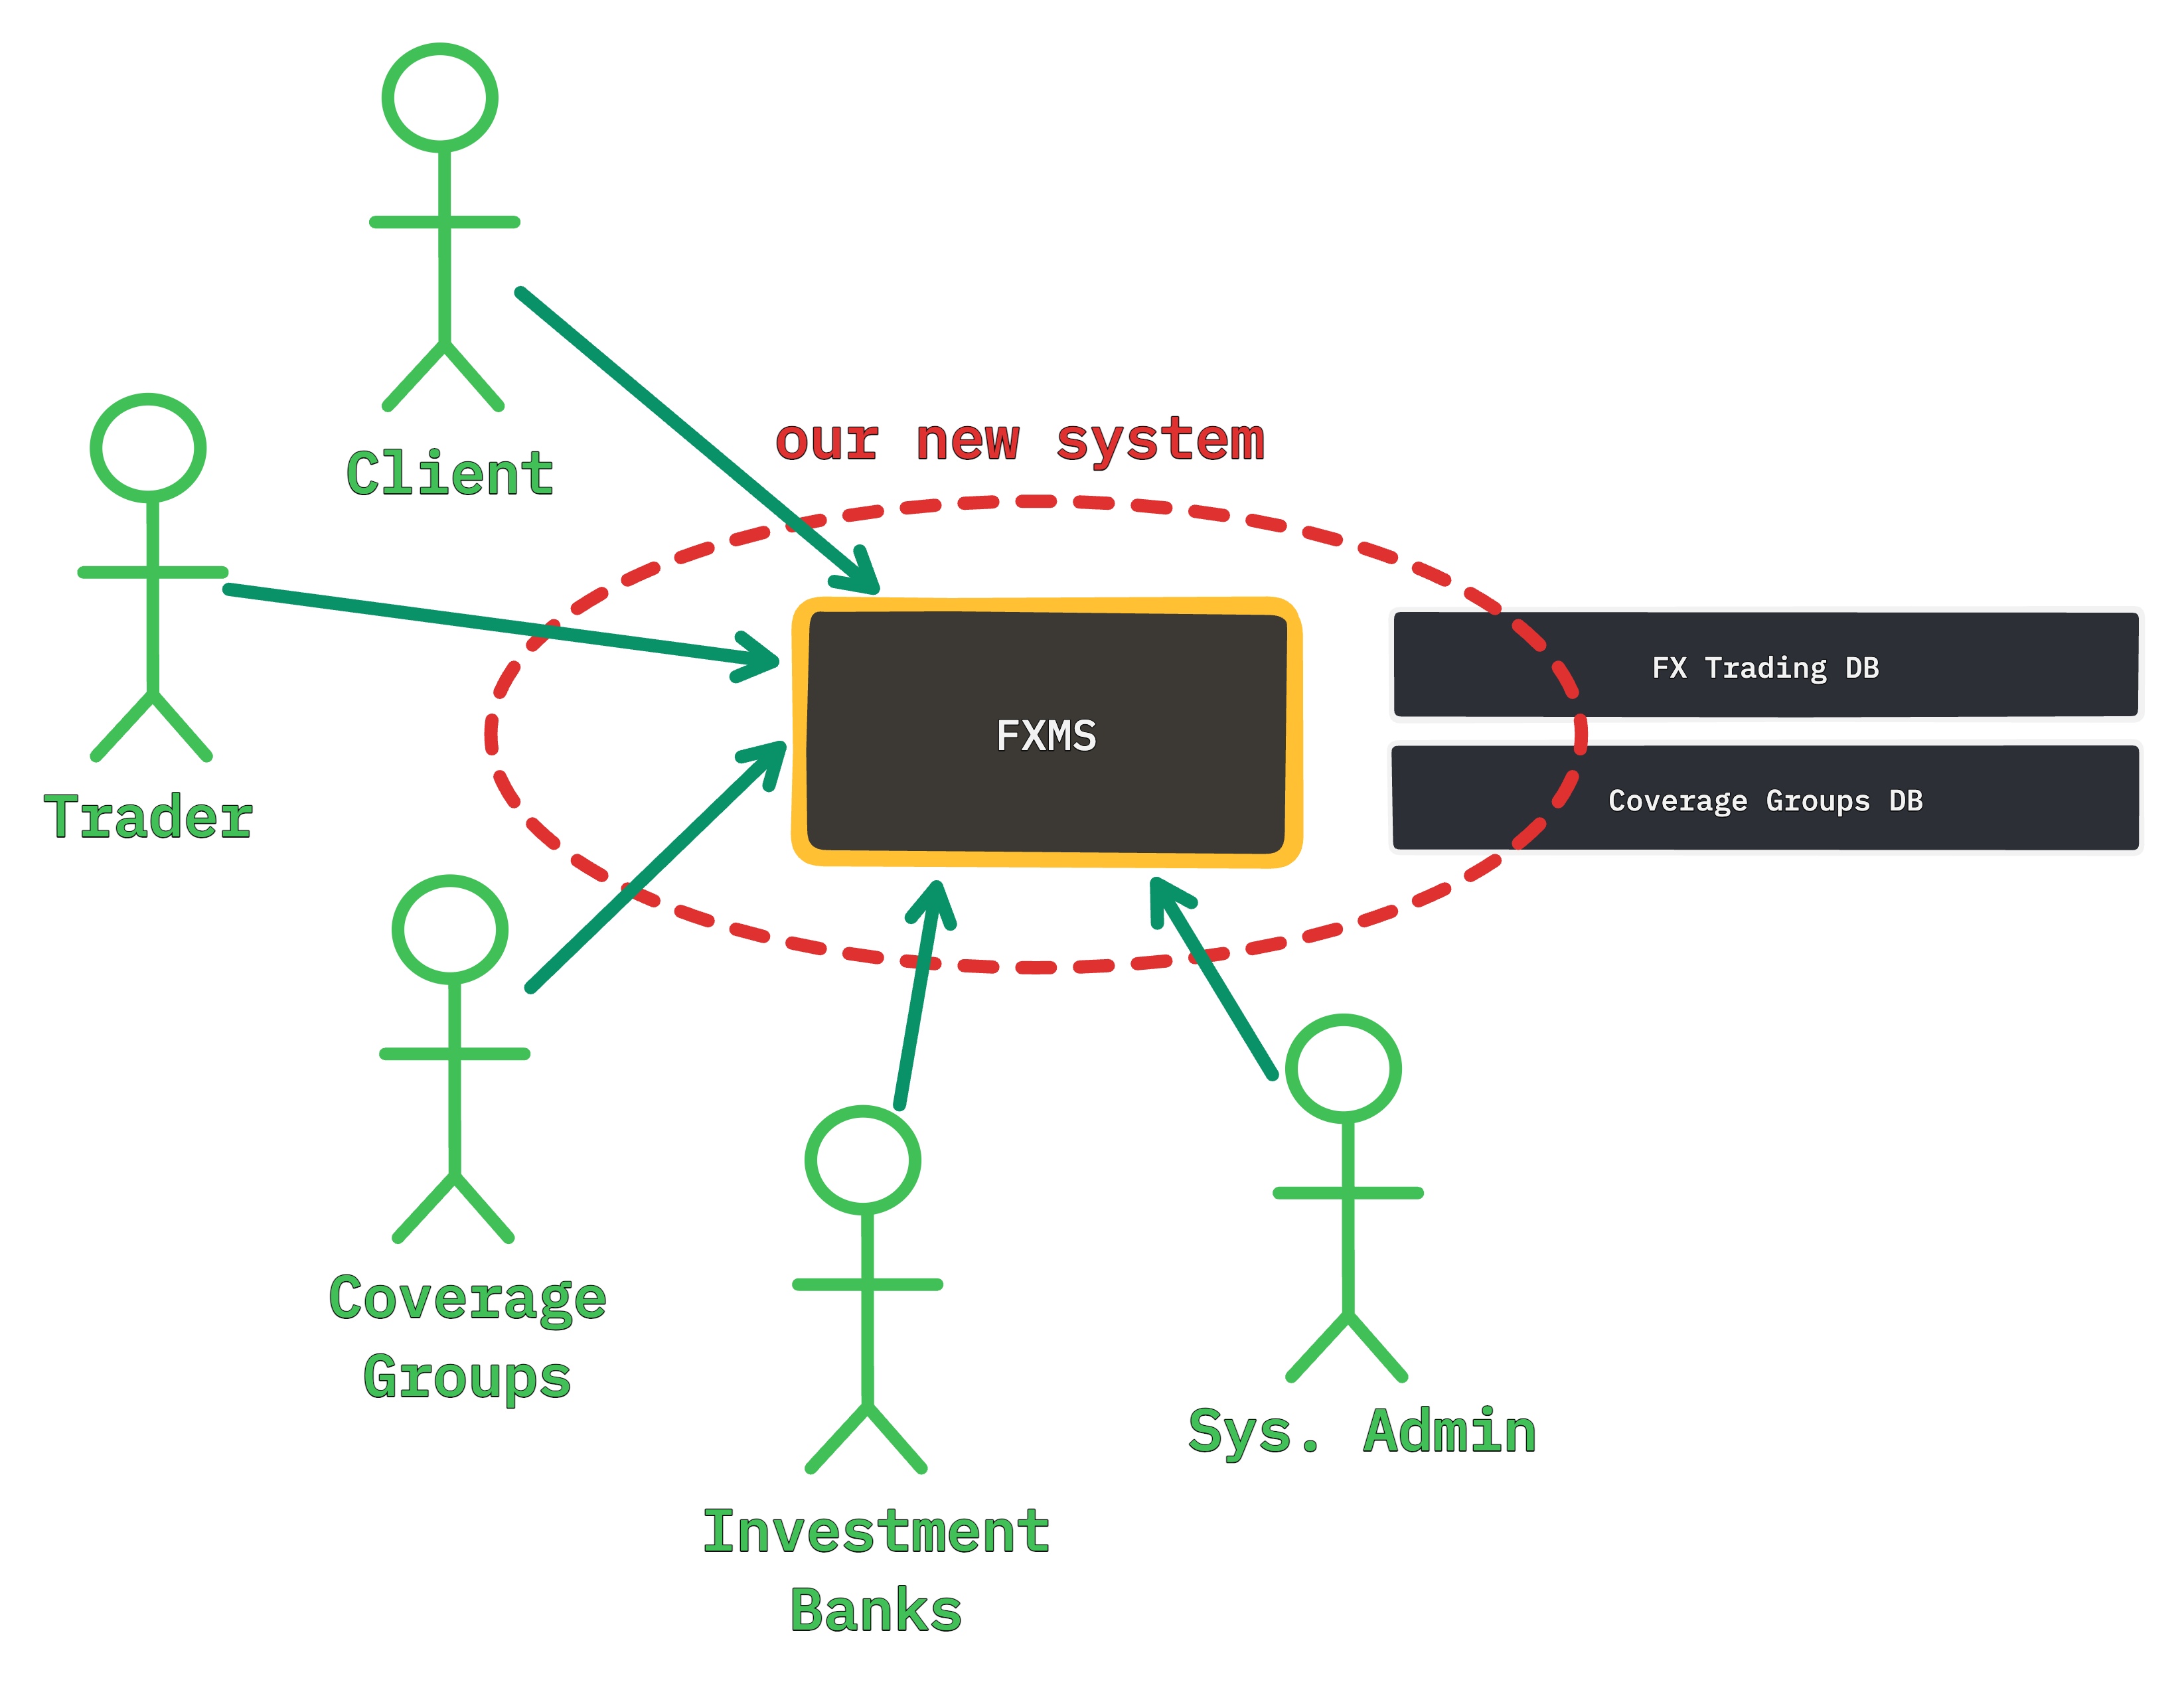
\includegraphics[width=\textwidth]{images/system-boundary.png}
    \caption{System Boundary of FXMS}
    \label{fig:system-boundary}
\end{figure}

\chapter{Functional Requirements}

Based on the information provided, the following functional requirements can be identified:
\begin{enumerate}
    \item The system shall allow managing accounts (insert, update, delete)
    \item The system shall allow managing trades (insert, update, delete)
    \item The system shall allow managing traders and coverage groups (assign traders to groups, move traders between groups)
    \item The system shall support different types of FX trades (spot, forward, swap, options)
    \item The system shall allow managing currencies and rates with a daily update of rates.
    \item The system shall calculate profit and loss for each trade
    \item The FXMS shall be able to search and retrieve specific trades using customizable filters (currencies, exchange rates, regions, dates).
    \item The FXMS shall be able to generate different types of reports (PnL, trade history, ...).
\end{enumerate}

\chapter{Non-Functional Requirements}

\begin{enumerate}
    \item Deployment: The system shall be deployed on Windows 10.
    \item Delivery Time: The system shall be delivered by the end of the current year.
    \item Performance: The system shall be able to execute a trade in a short time (50 trades per second).
    \item Availability: The system shall be available between 6am to 6pm. Bugs shall be resolved within 30 minutes maxmimum in those hours.
    \item Security: The system shall have role-based access control to manage users access to data (such as identity of customers, PnL, ...) and there should be strict access control to the system.
    \item Reliability: The system shall be reliable and available 99.9\% of the time.
    \item Usability: The system shall be easy to use and user friendly.
\end{enumerate}

\chapter{UC Model}

\section{Use Case Diagram}

The use case diagram of the FXMS is shown in Figure \ref{fig:use-case-diagram}. The diagrams shows the functional requirements of the sytem layed out at use cases so that it is easier to comprehed.

\begin{figure}[h!]
    \centering
    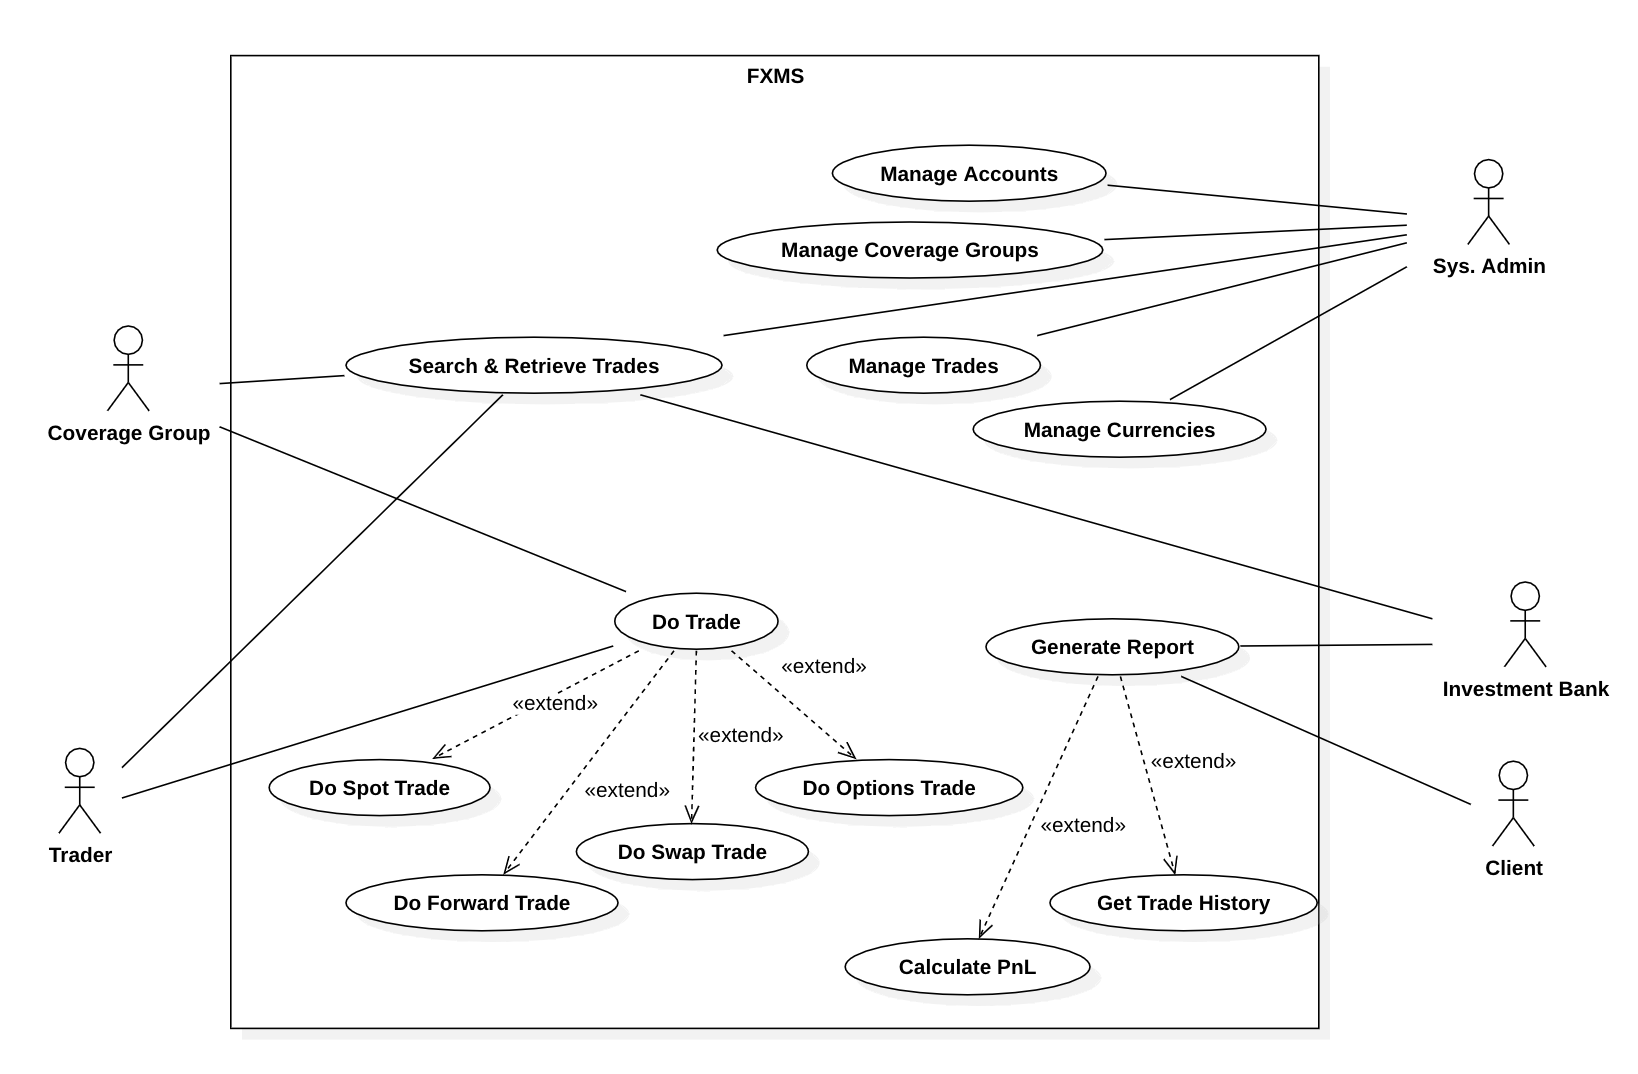
\includegraphics[width=\textwidth]{images/use-case-diagram.png}
    \caption{Use Case Diagram of FXMS}
    \label{fig:use-case-diagram}
\end{figure}

\section{Use Cases Descriptions}

\begin{figure}[h!]
    \centering
    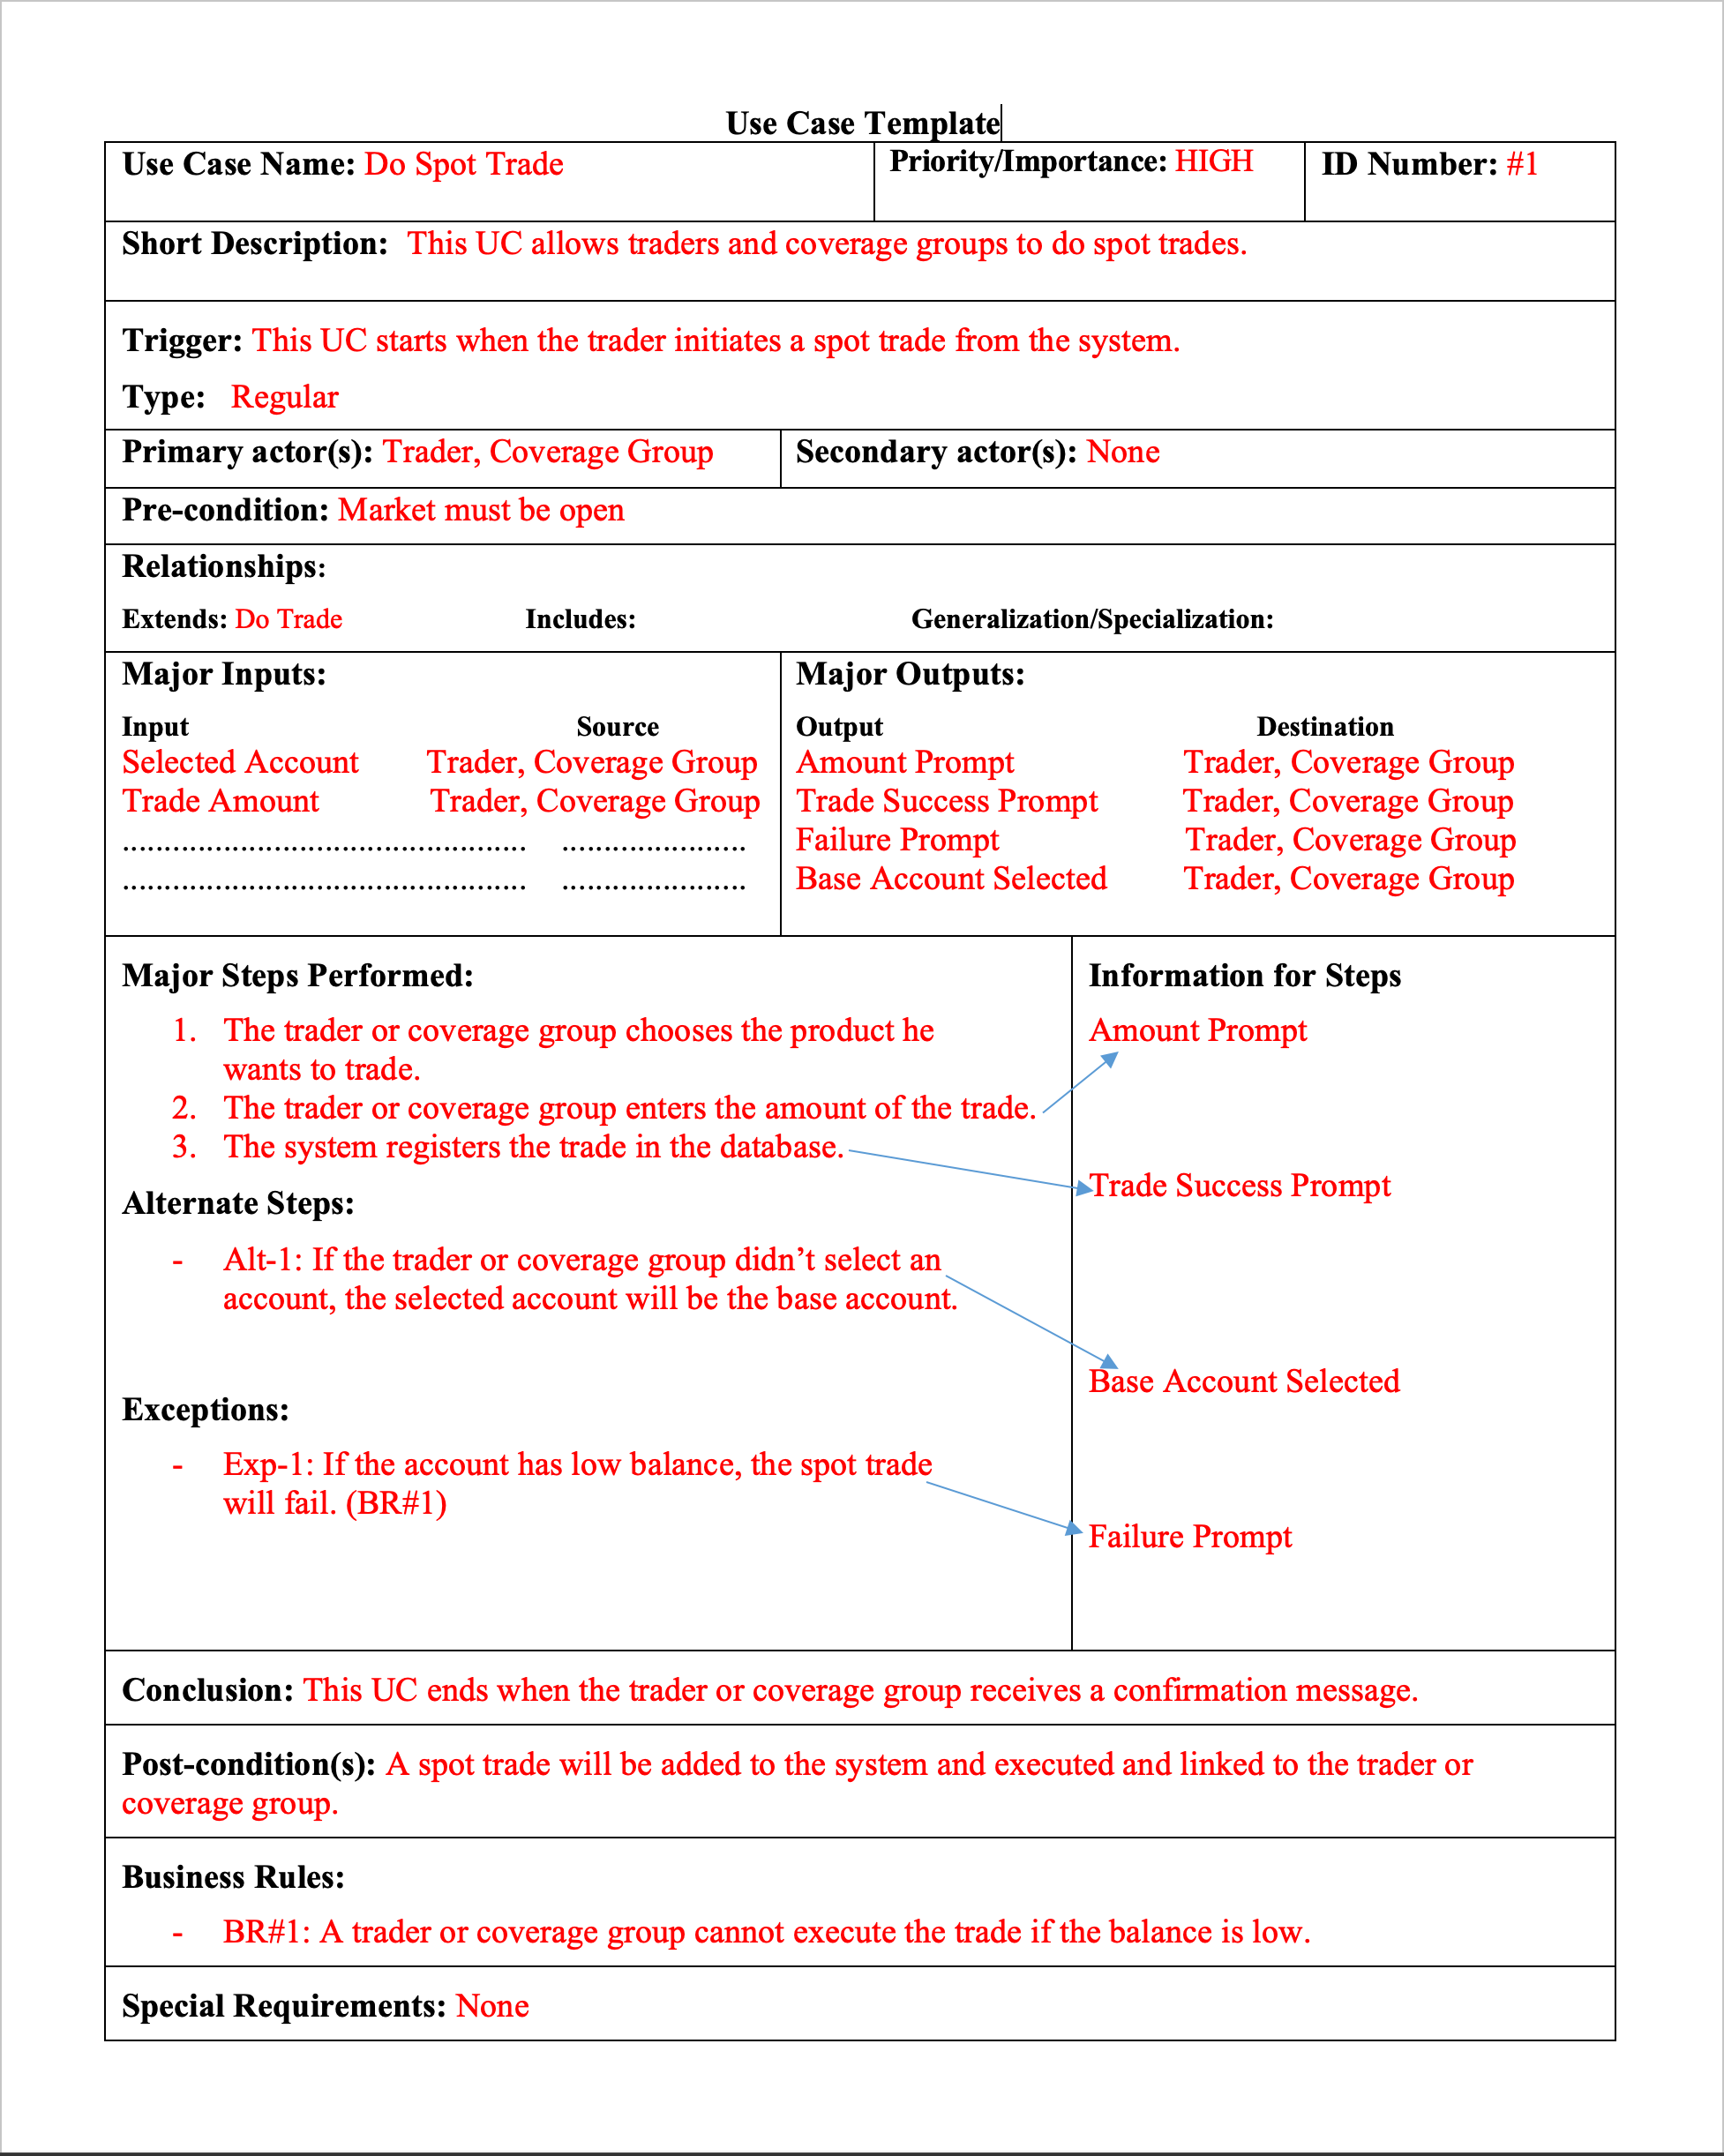
\includegraphics[width=\textwidth]{images/uc/1-do-spot-trade.png}
    \caption{Do Spot Trade}
    \label{fig:1-do-spot-trade}
\end{figure}

\begin{figure}[h!]
    \centering
    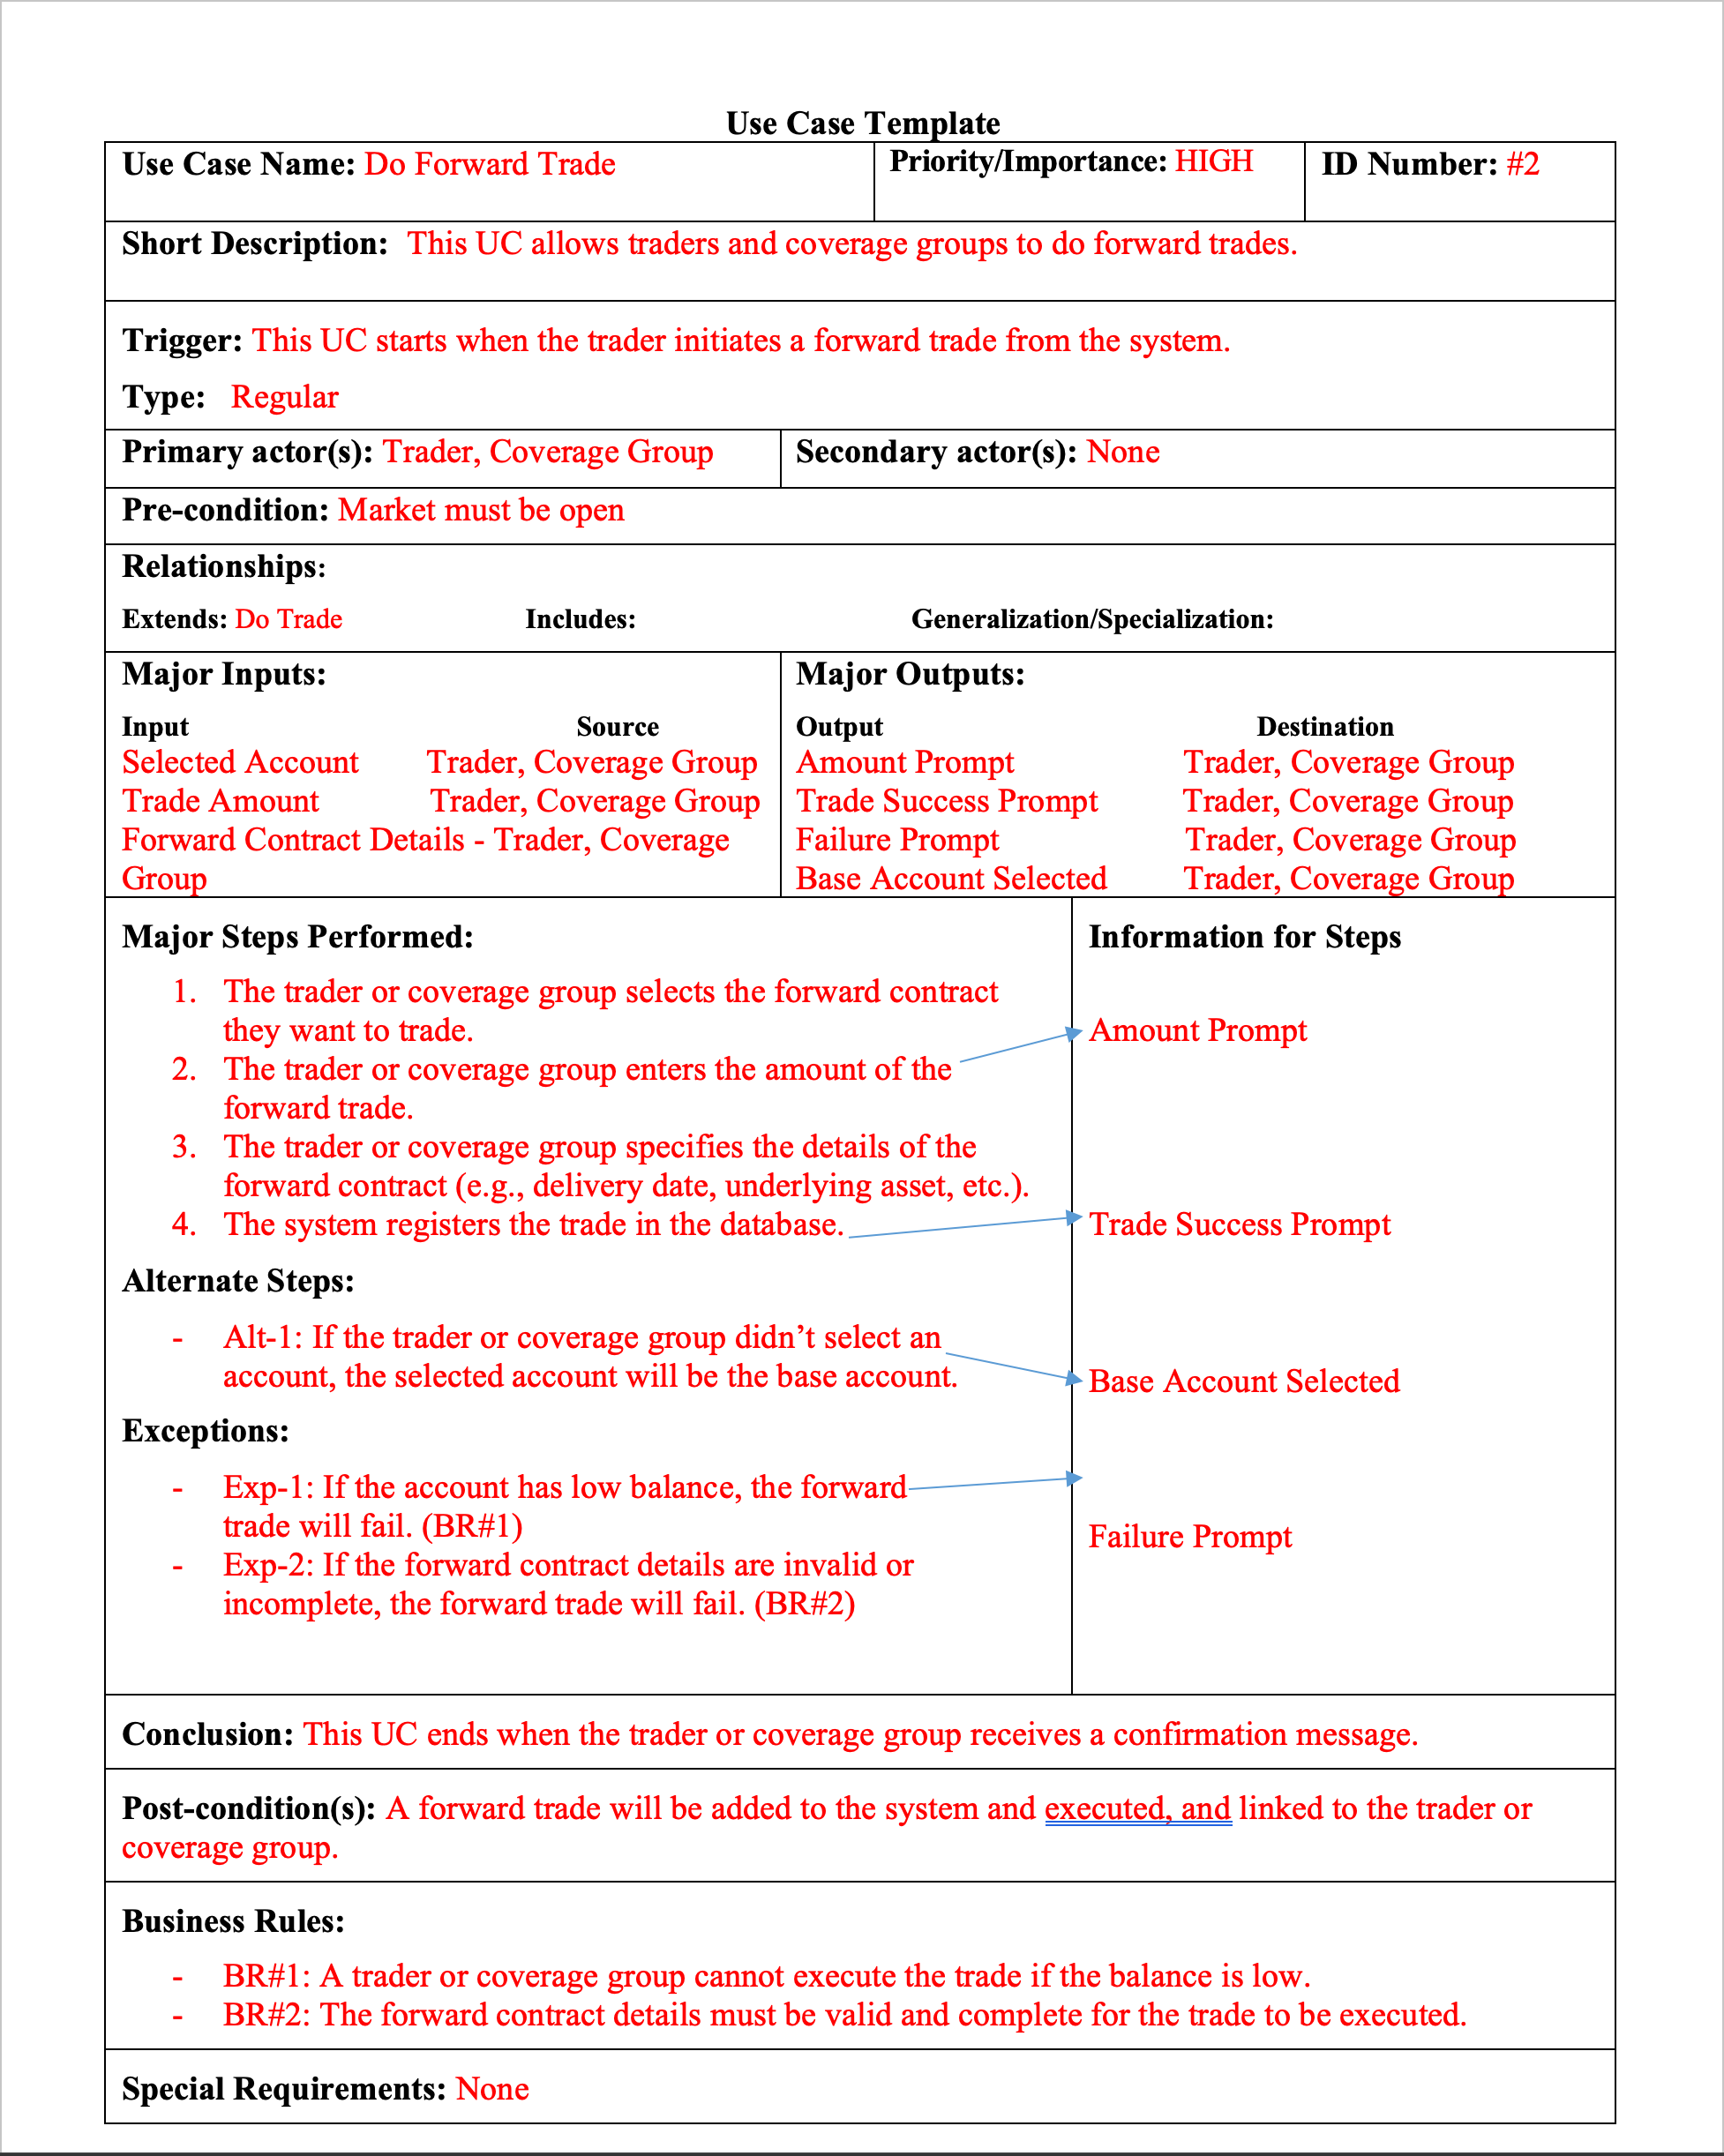
\includegraphics[width=\textwidth]{images/uc/2-do-forward-trade.png}
    \caption{Do Forward Trade}
    \label{fig:2-do-forward-trade}
\end{figure}

\begin{figure}[h!]
    \centering
    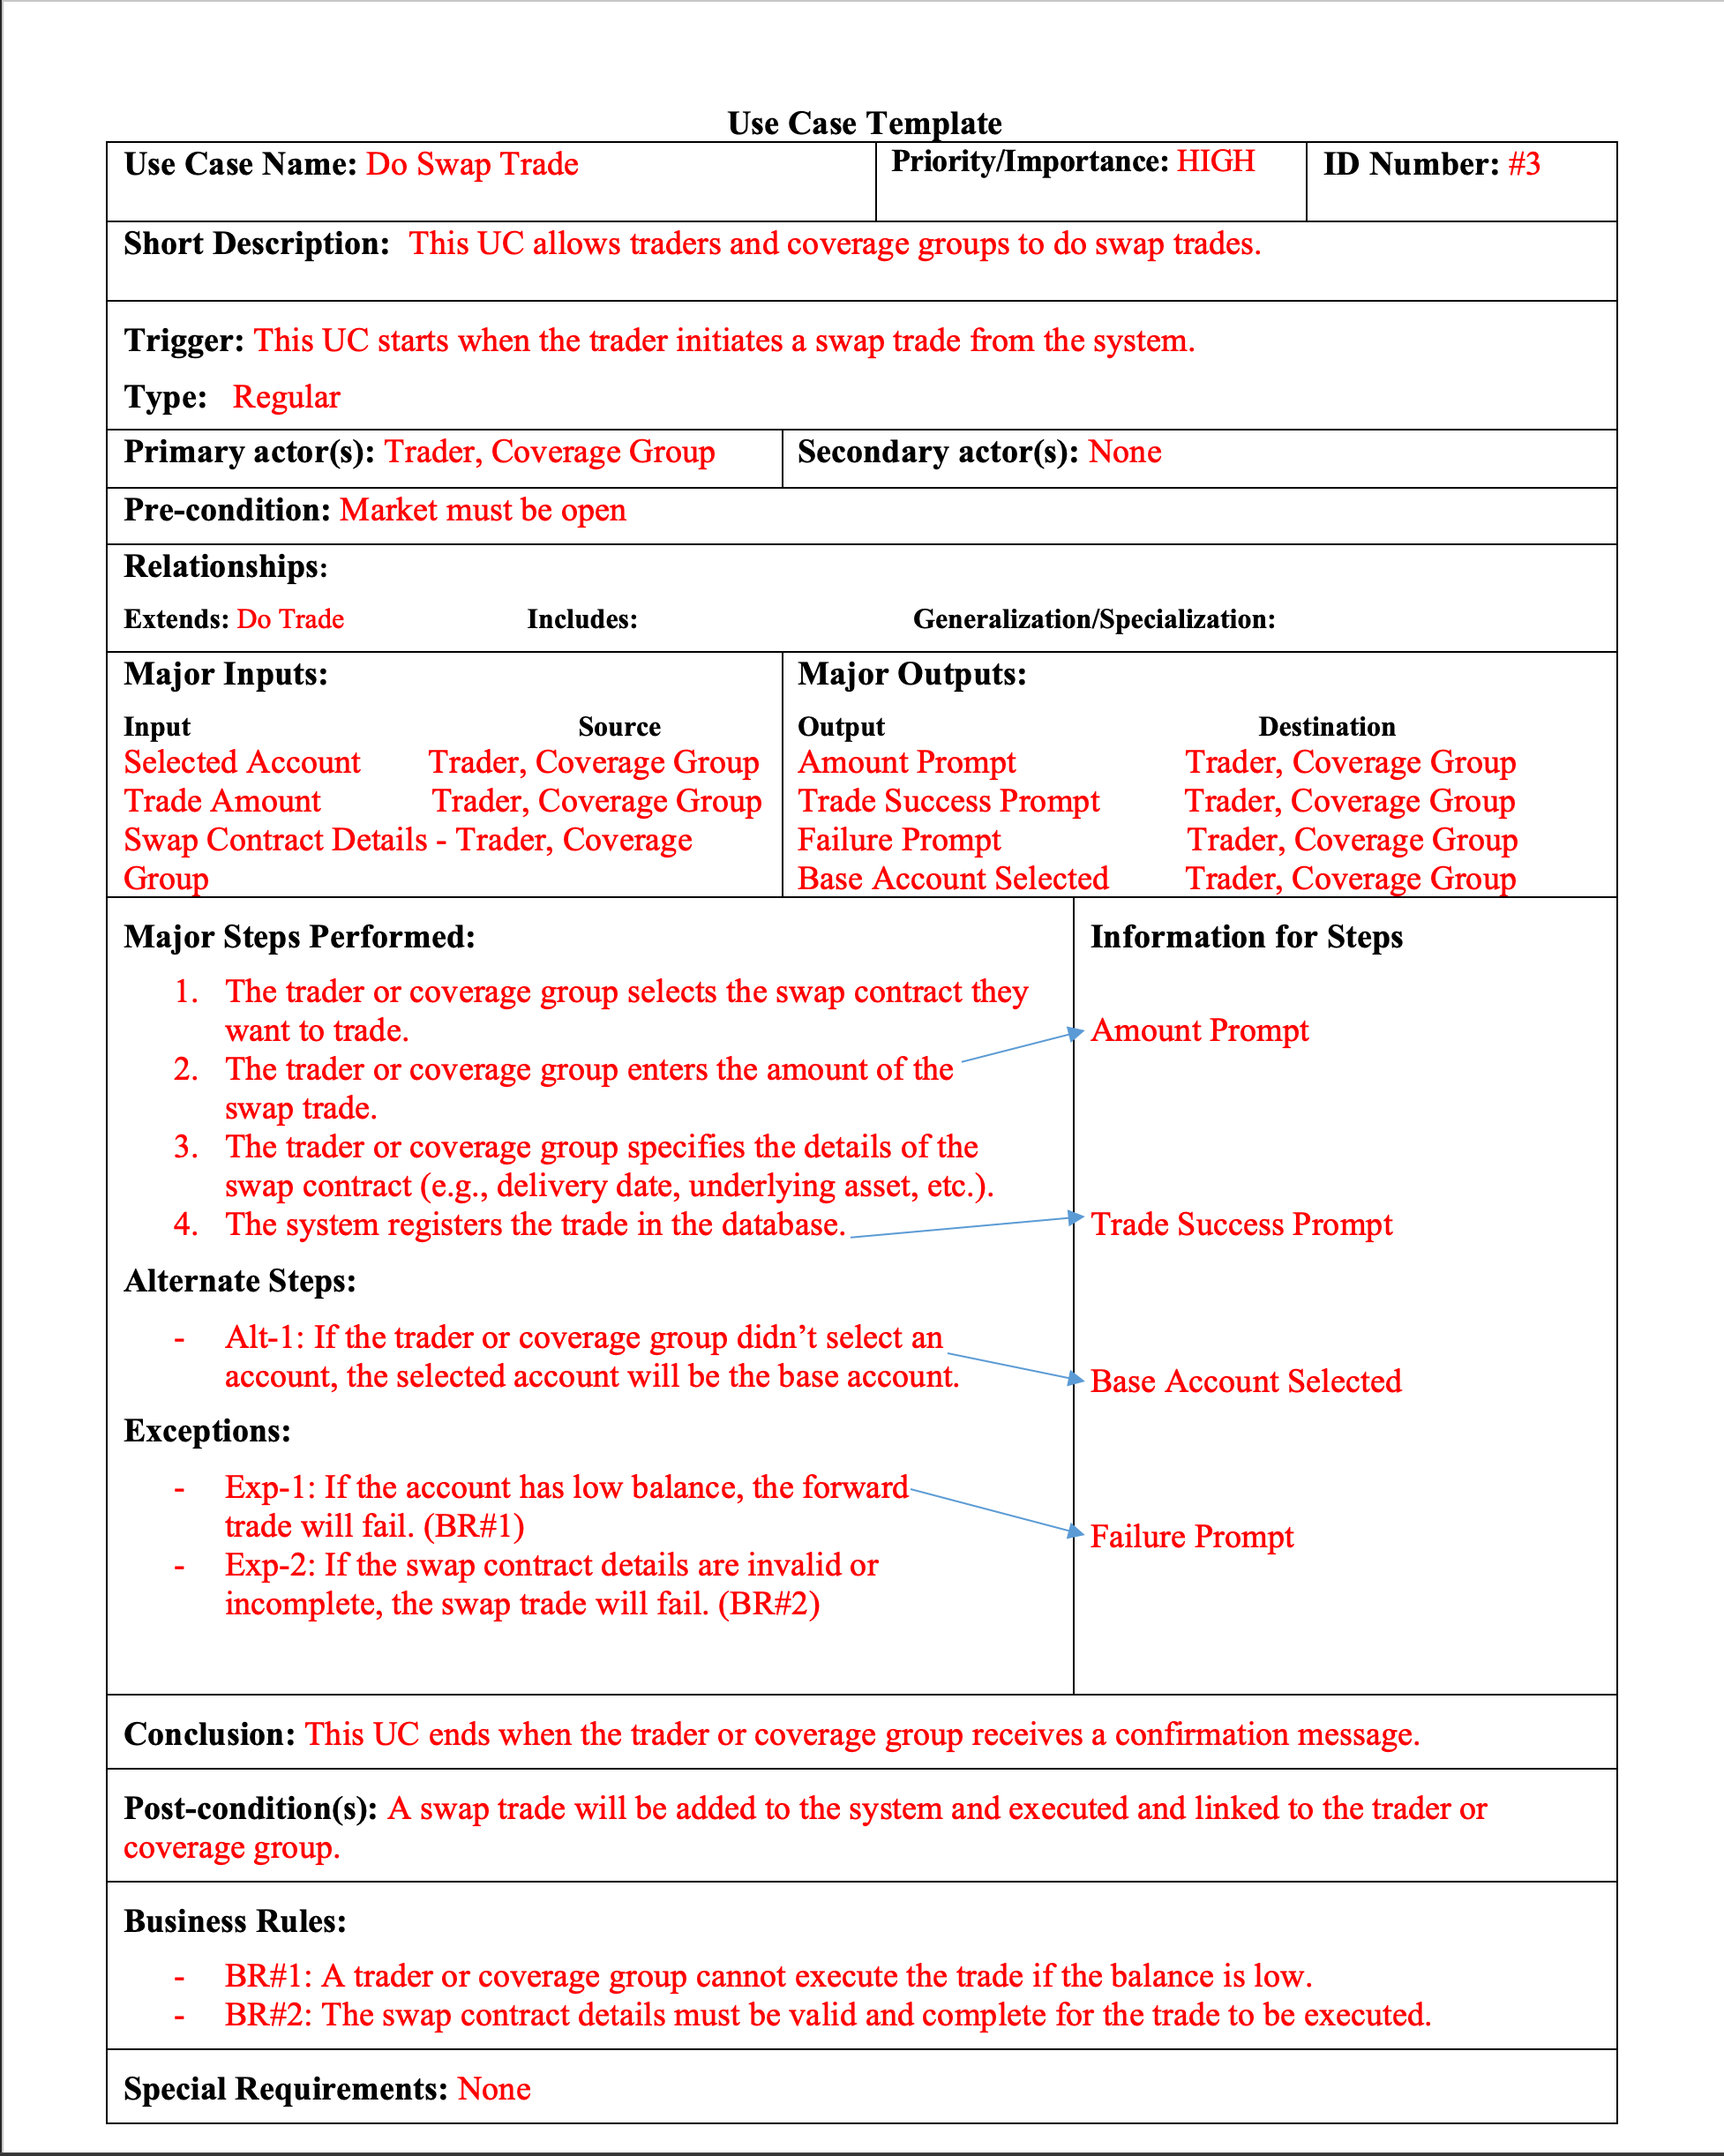
\includegraphics[width=\textwidth]{images/uc/3-do-swap-trade.png}
    \caption{Do Swap Trade}
    \label{fig:3-do-swap-trade}
\end{figure}

\begin{figure}[h!]
    \centering
    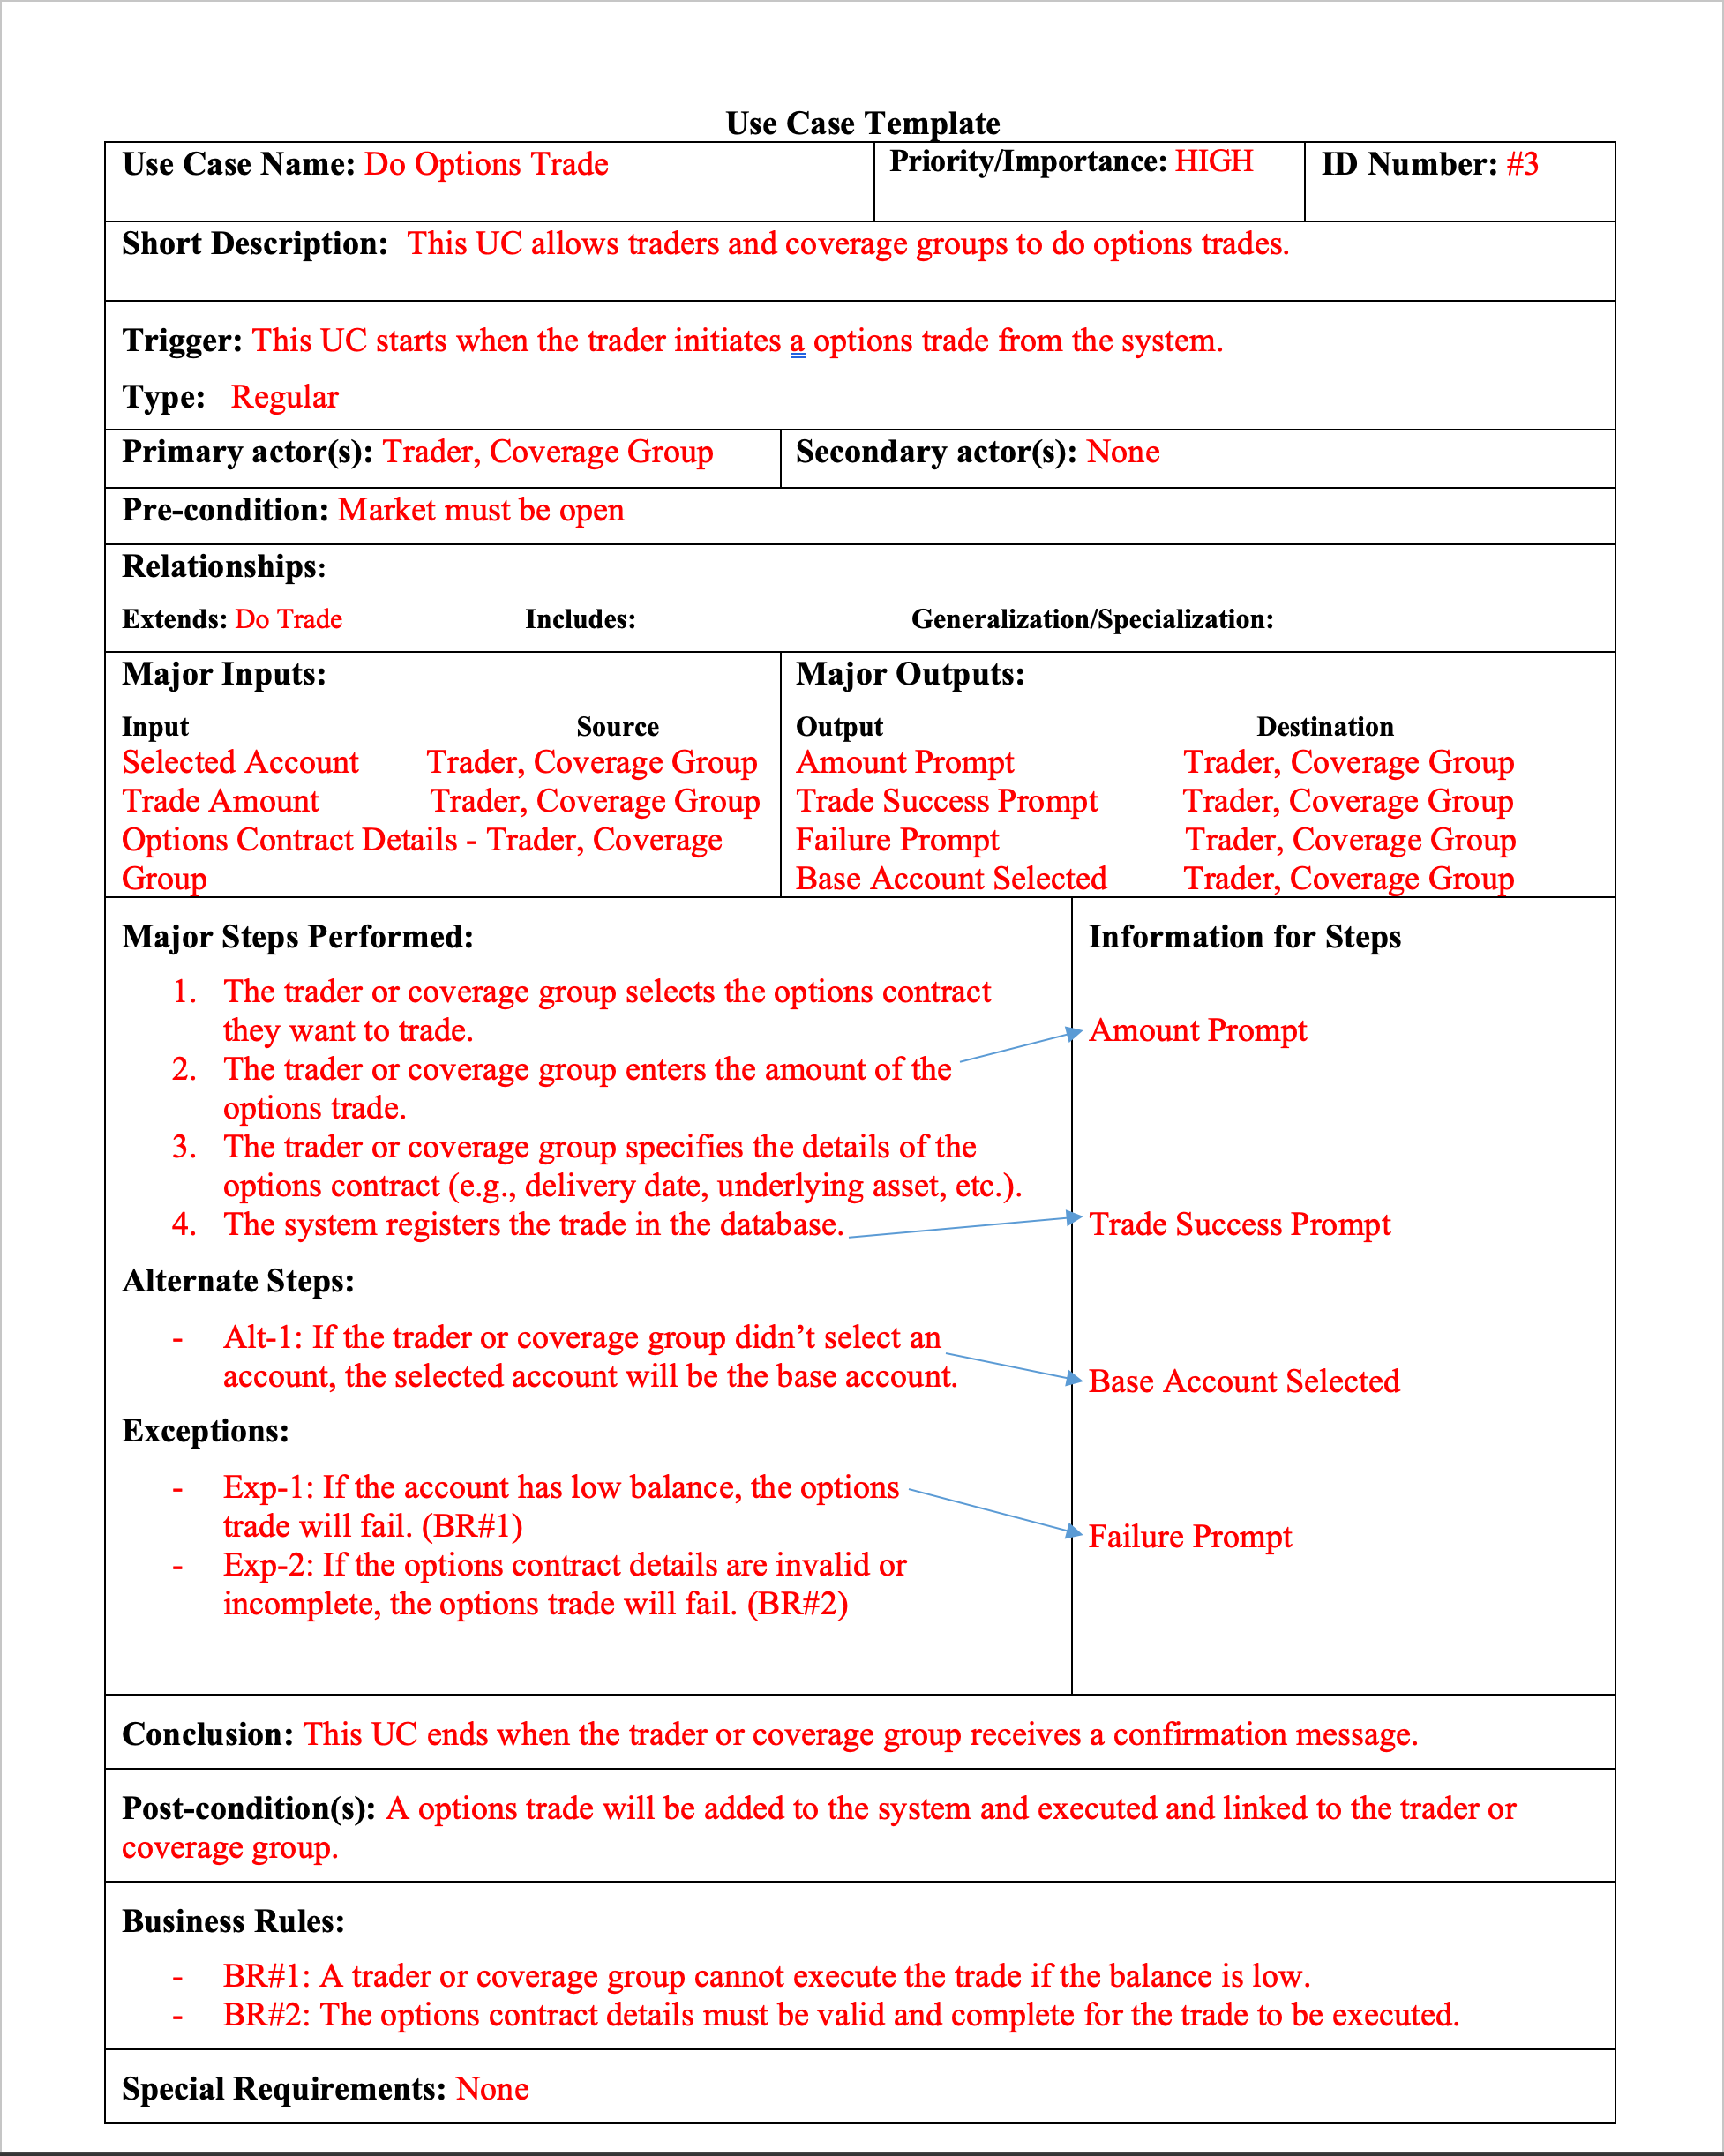
\includegraphics[width=\textwidth]{images/uc/4-do-options-trade.png}
    \caption{Do Options Trade}
    \label{fig:4-do-options-trade}
\end{figure}

\begin{figure}[h!]
    \centering
    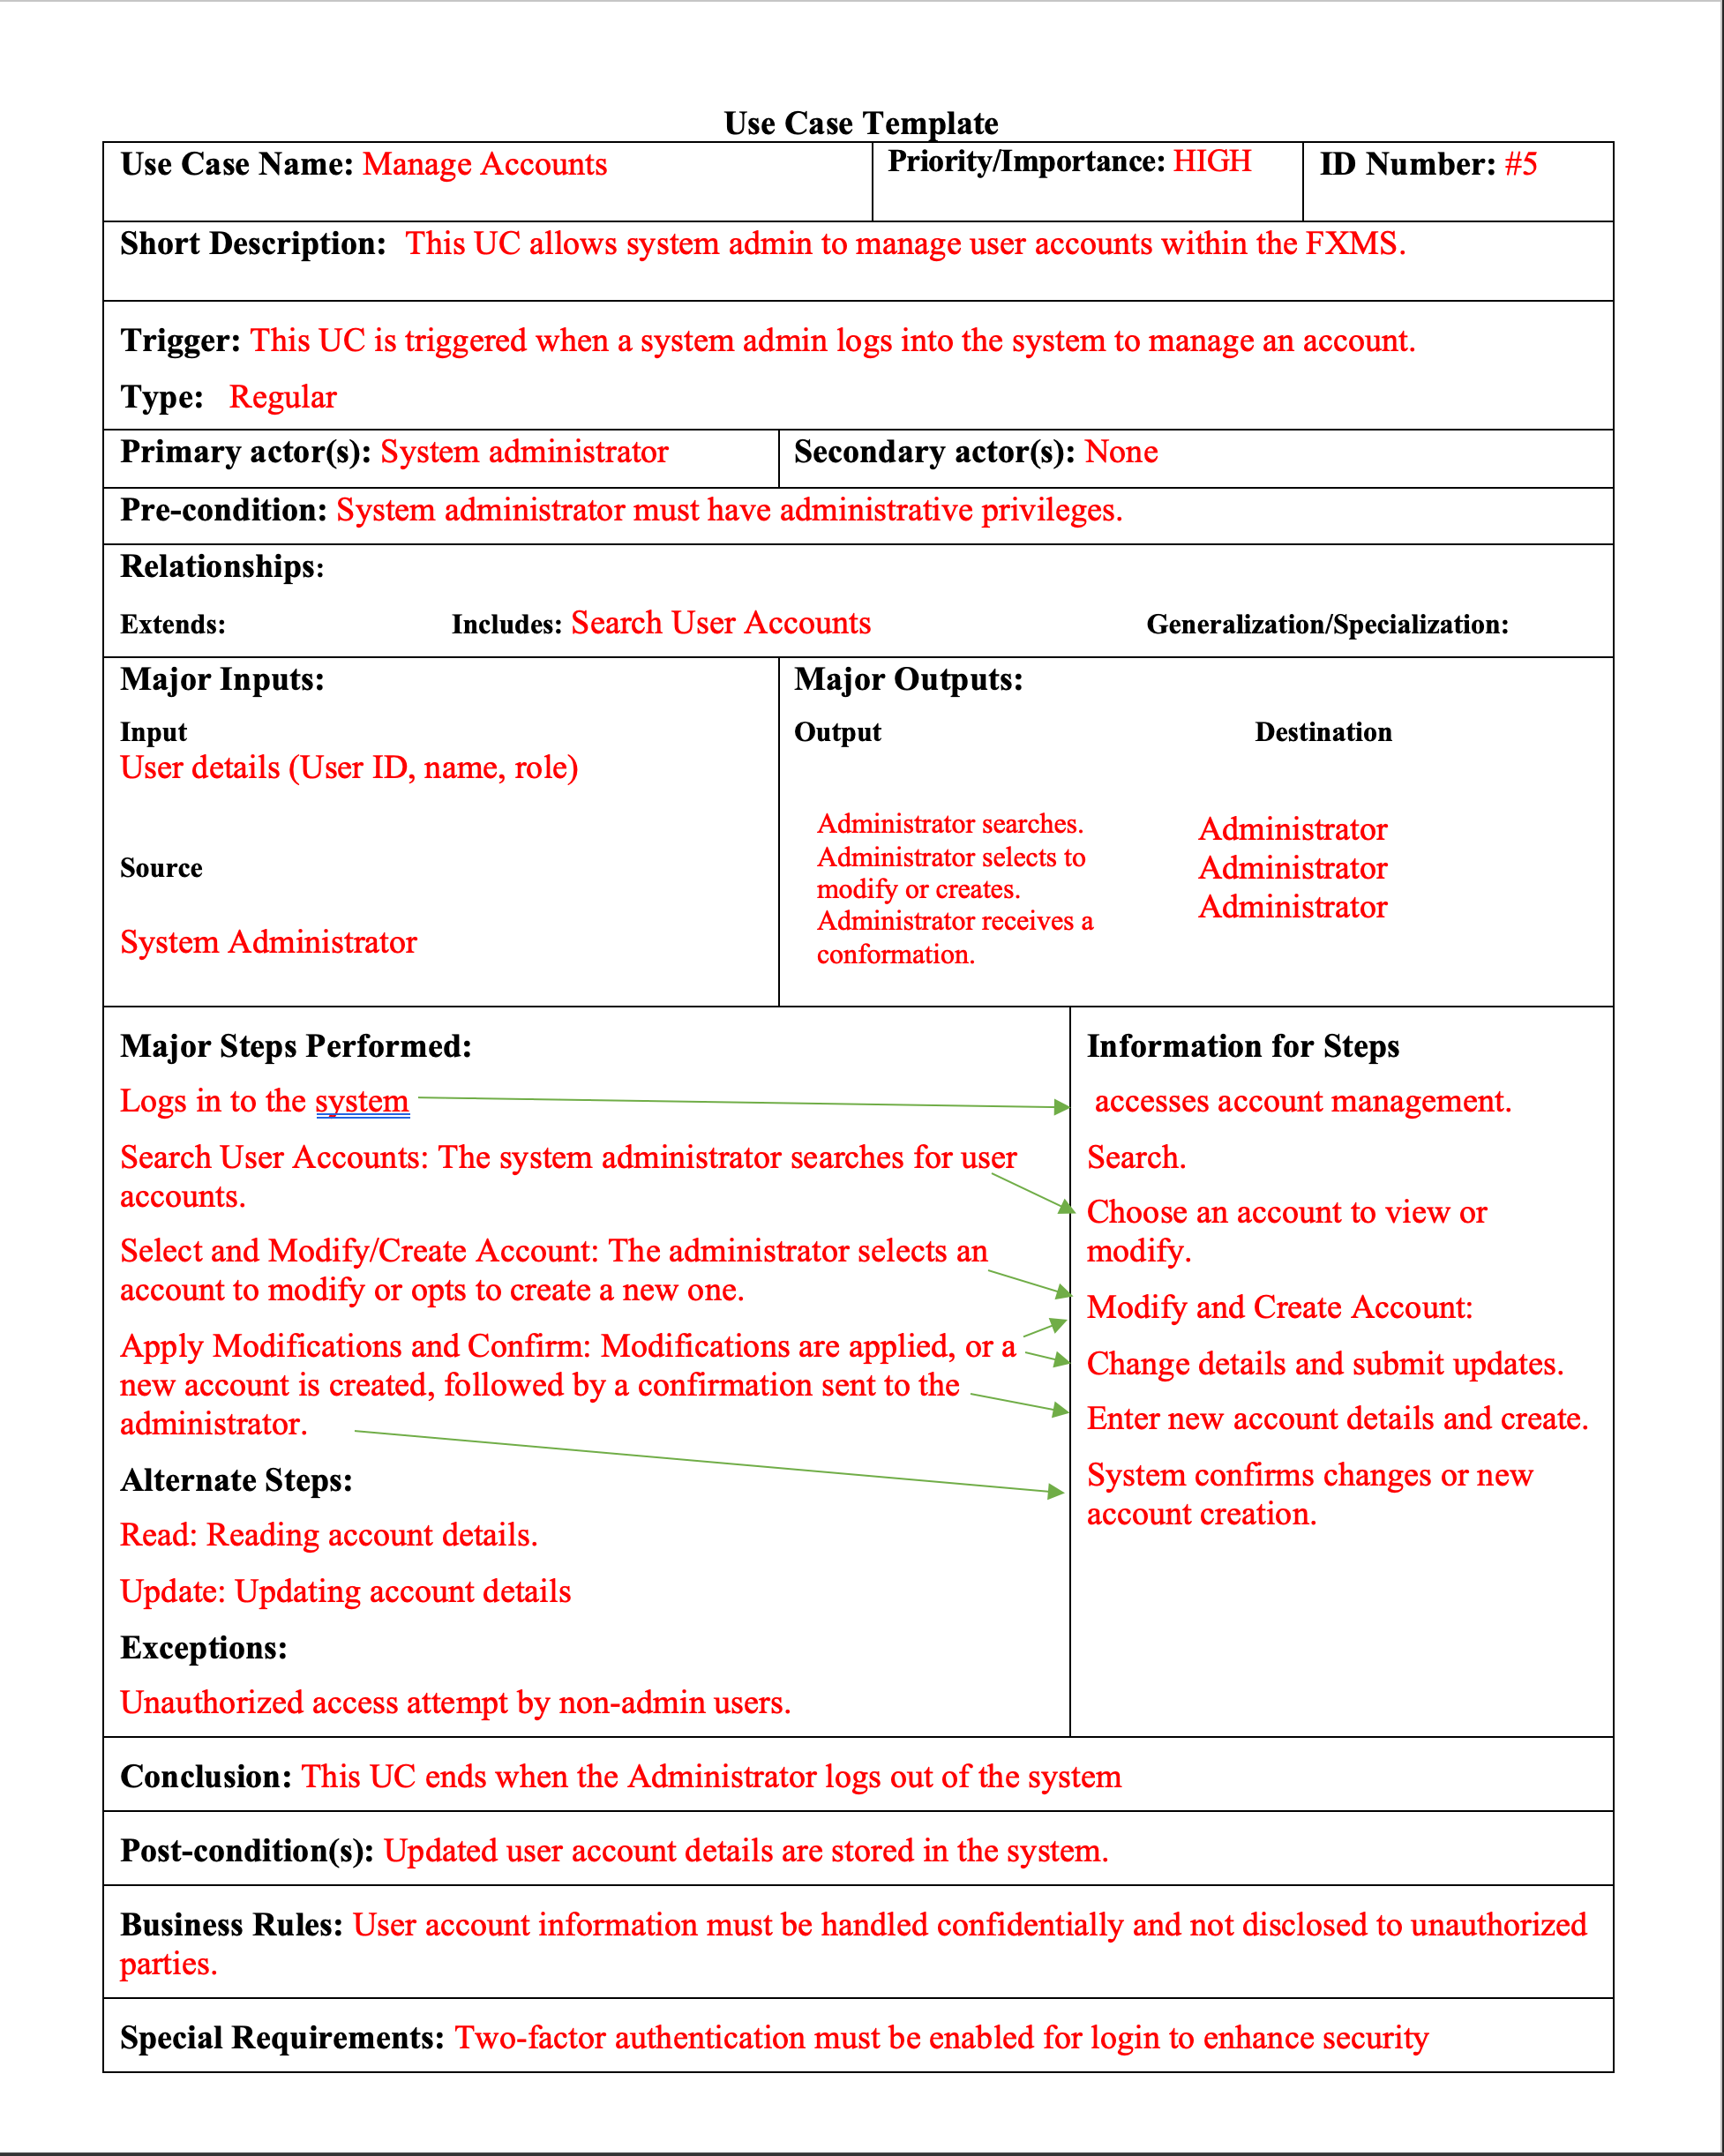
\includegraphics[width=\textwidth]{images/uc/5-manage-accounts.png}
    \caption{Manage Accounts}
    \label{fig:5-manage-accounts}
\end{figure}

\begin{figure}[h!]
    \centering
    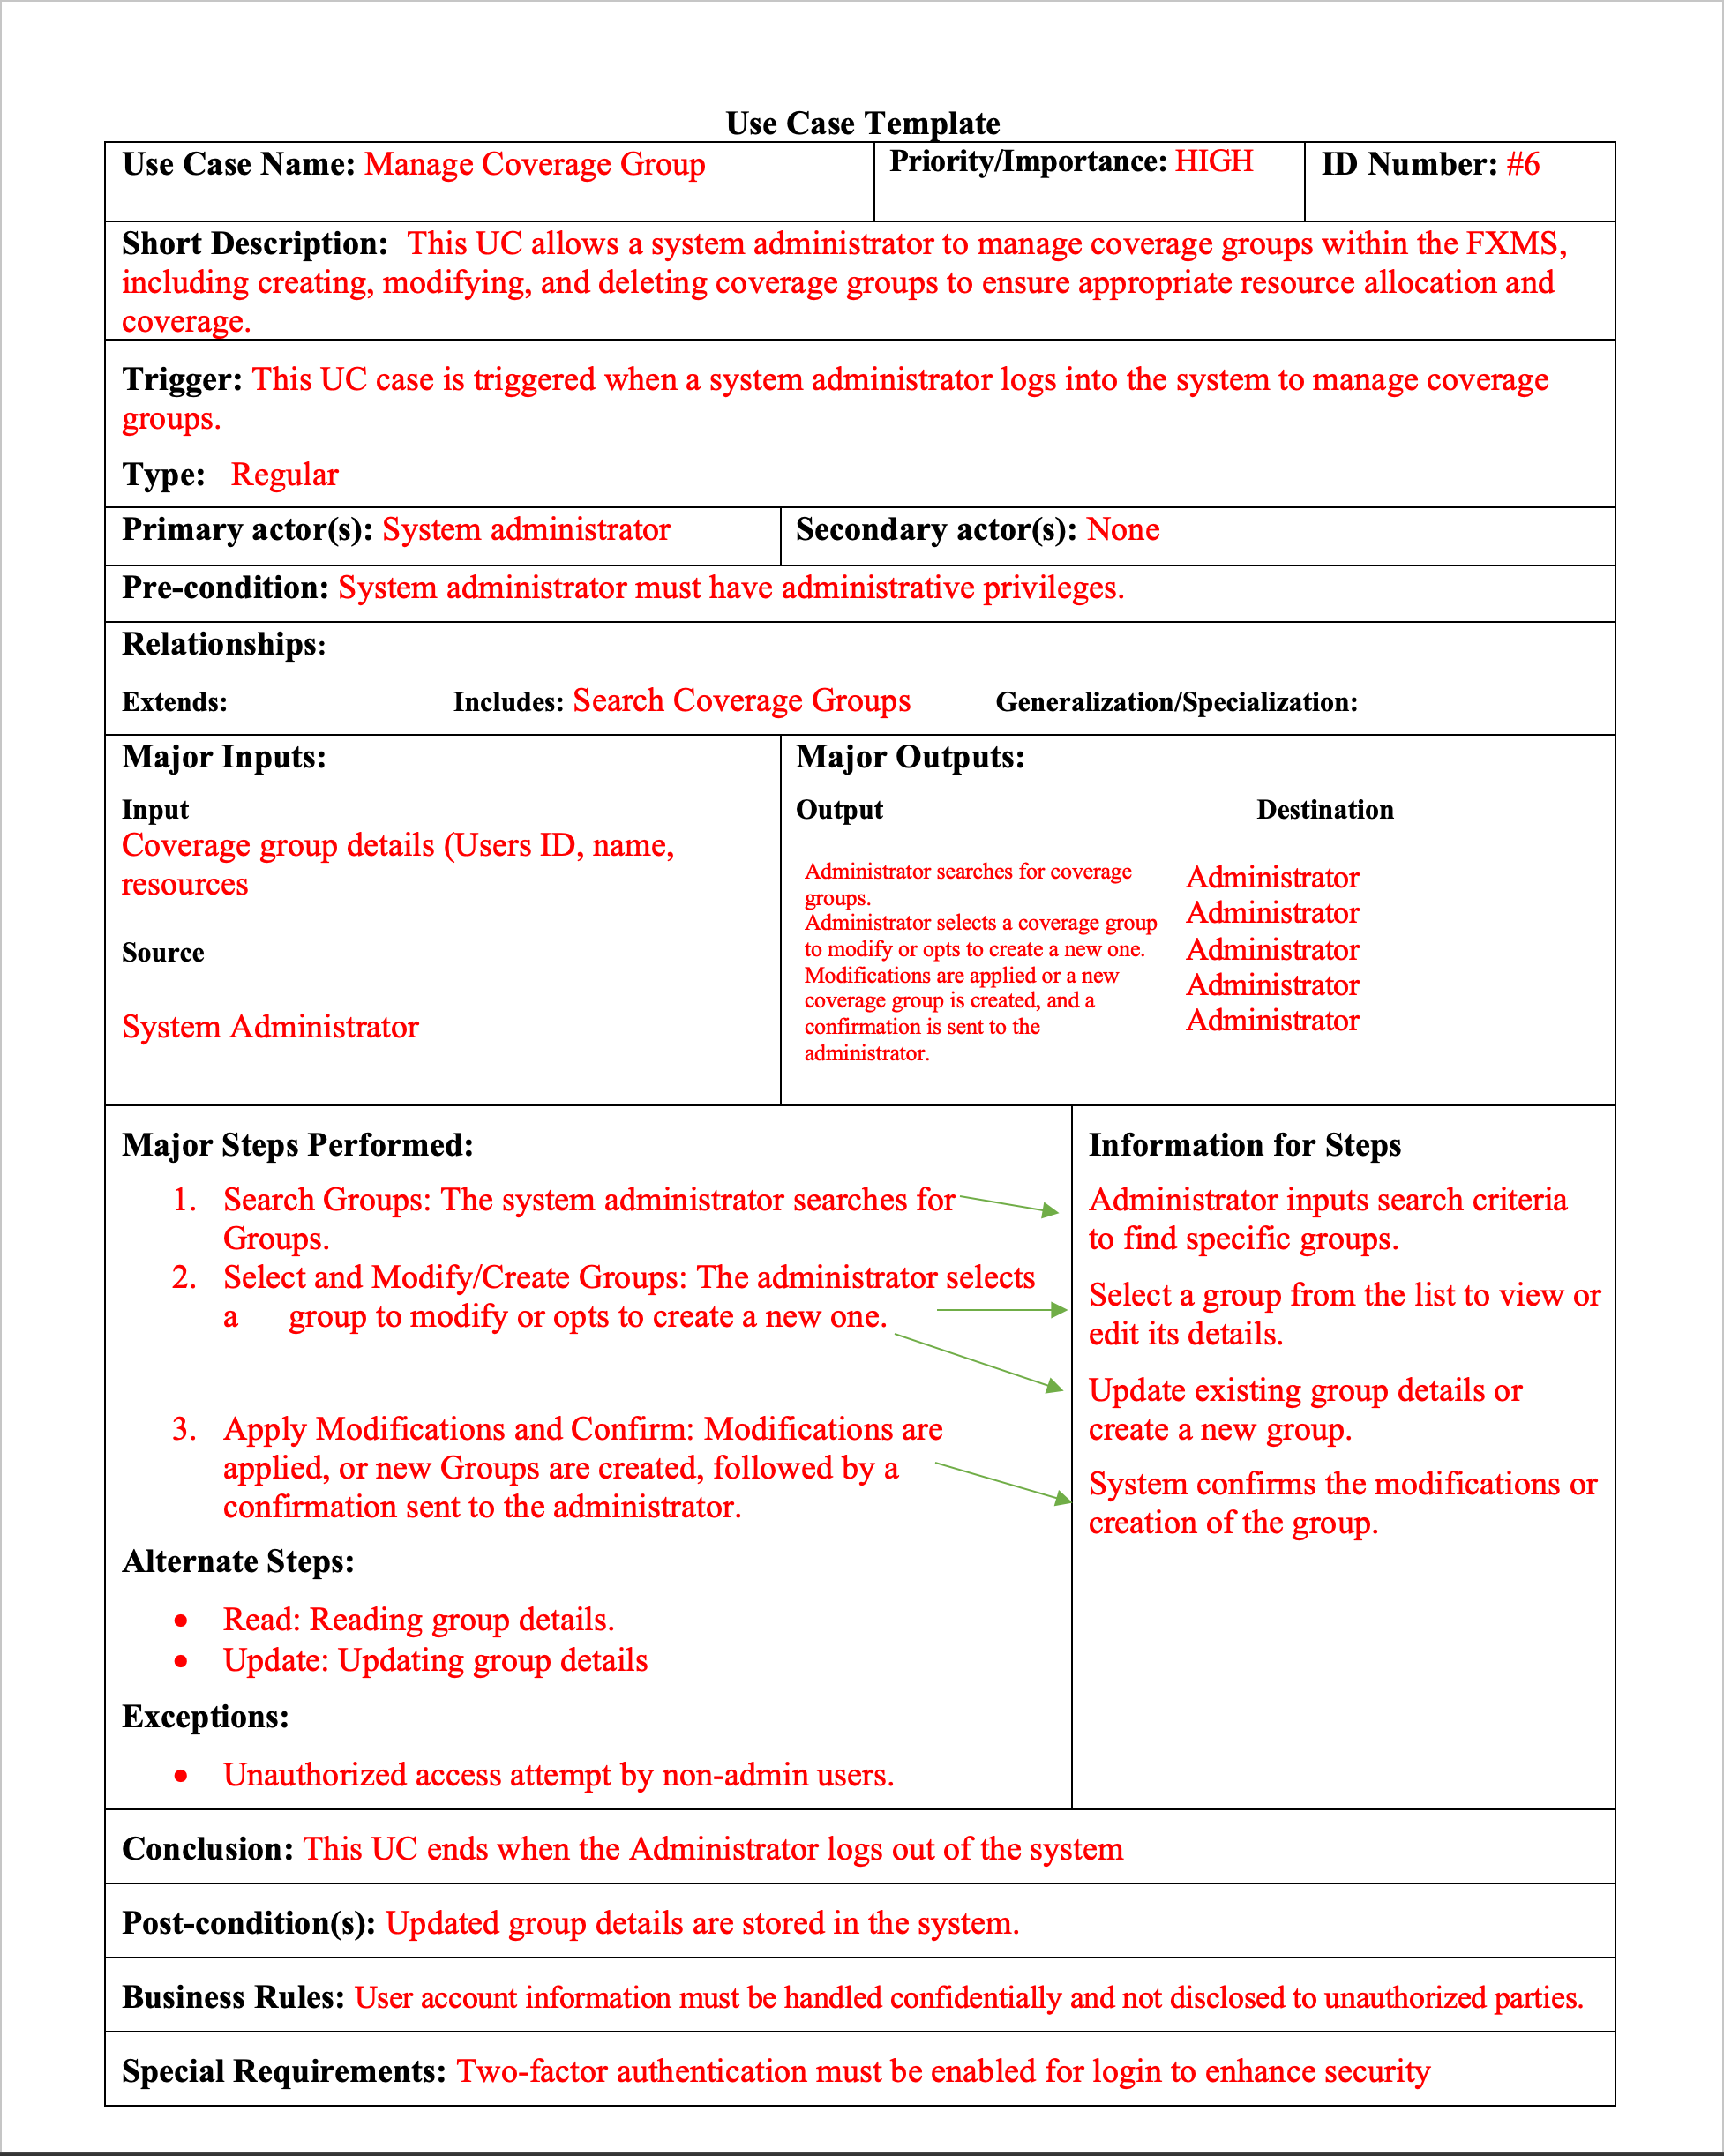
\includegraphics[width=\textwidth]{images/uc/6-manage-coverage-groups.png}
    \caption{Manage Coverage Groups}
    \label{fig:6-manage-coverage-groups}
\end{figure}

\begin{figure}[h!]
    \centering
    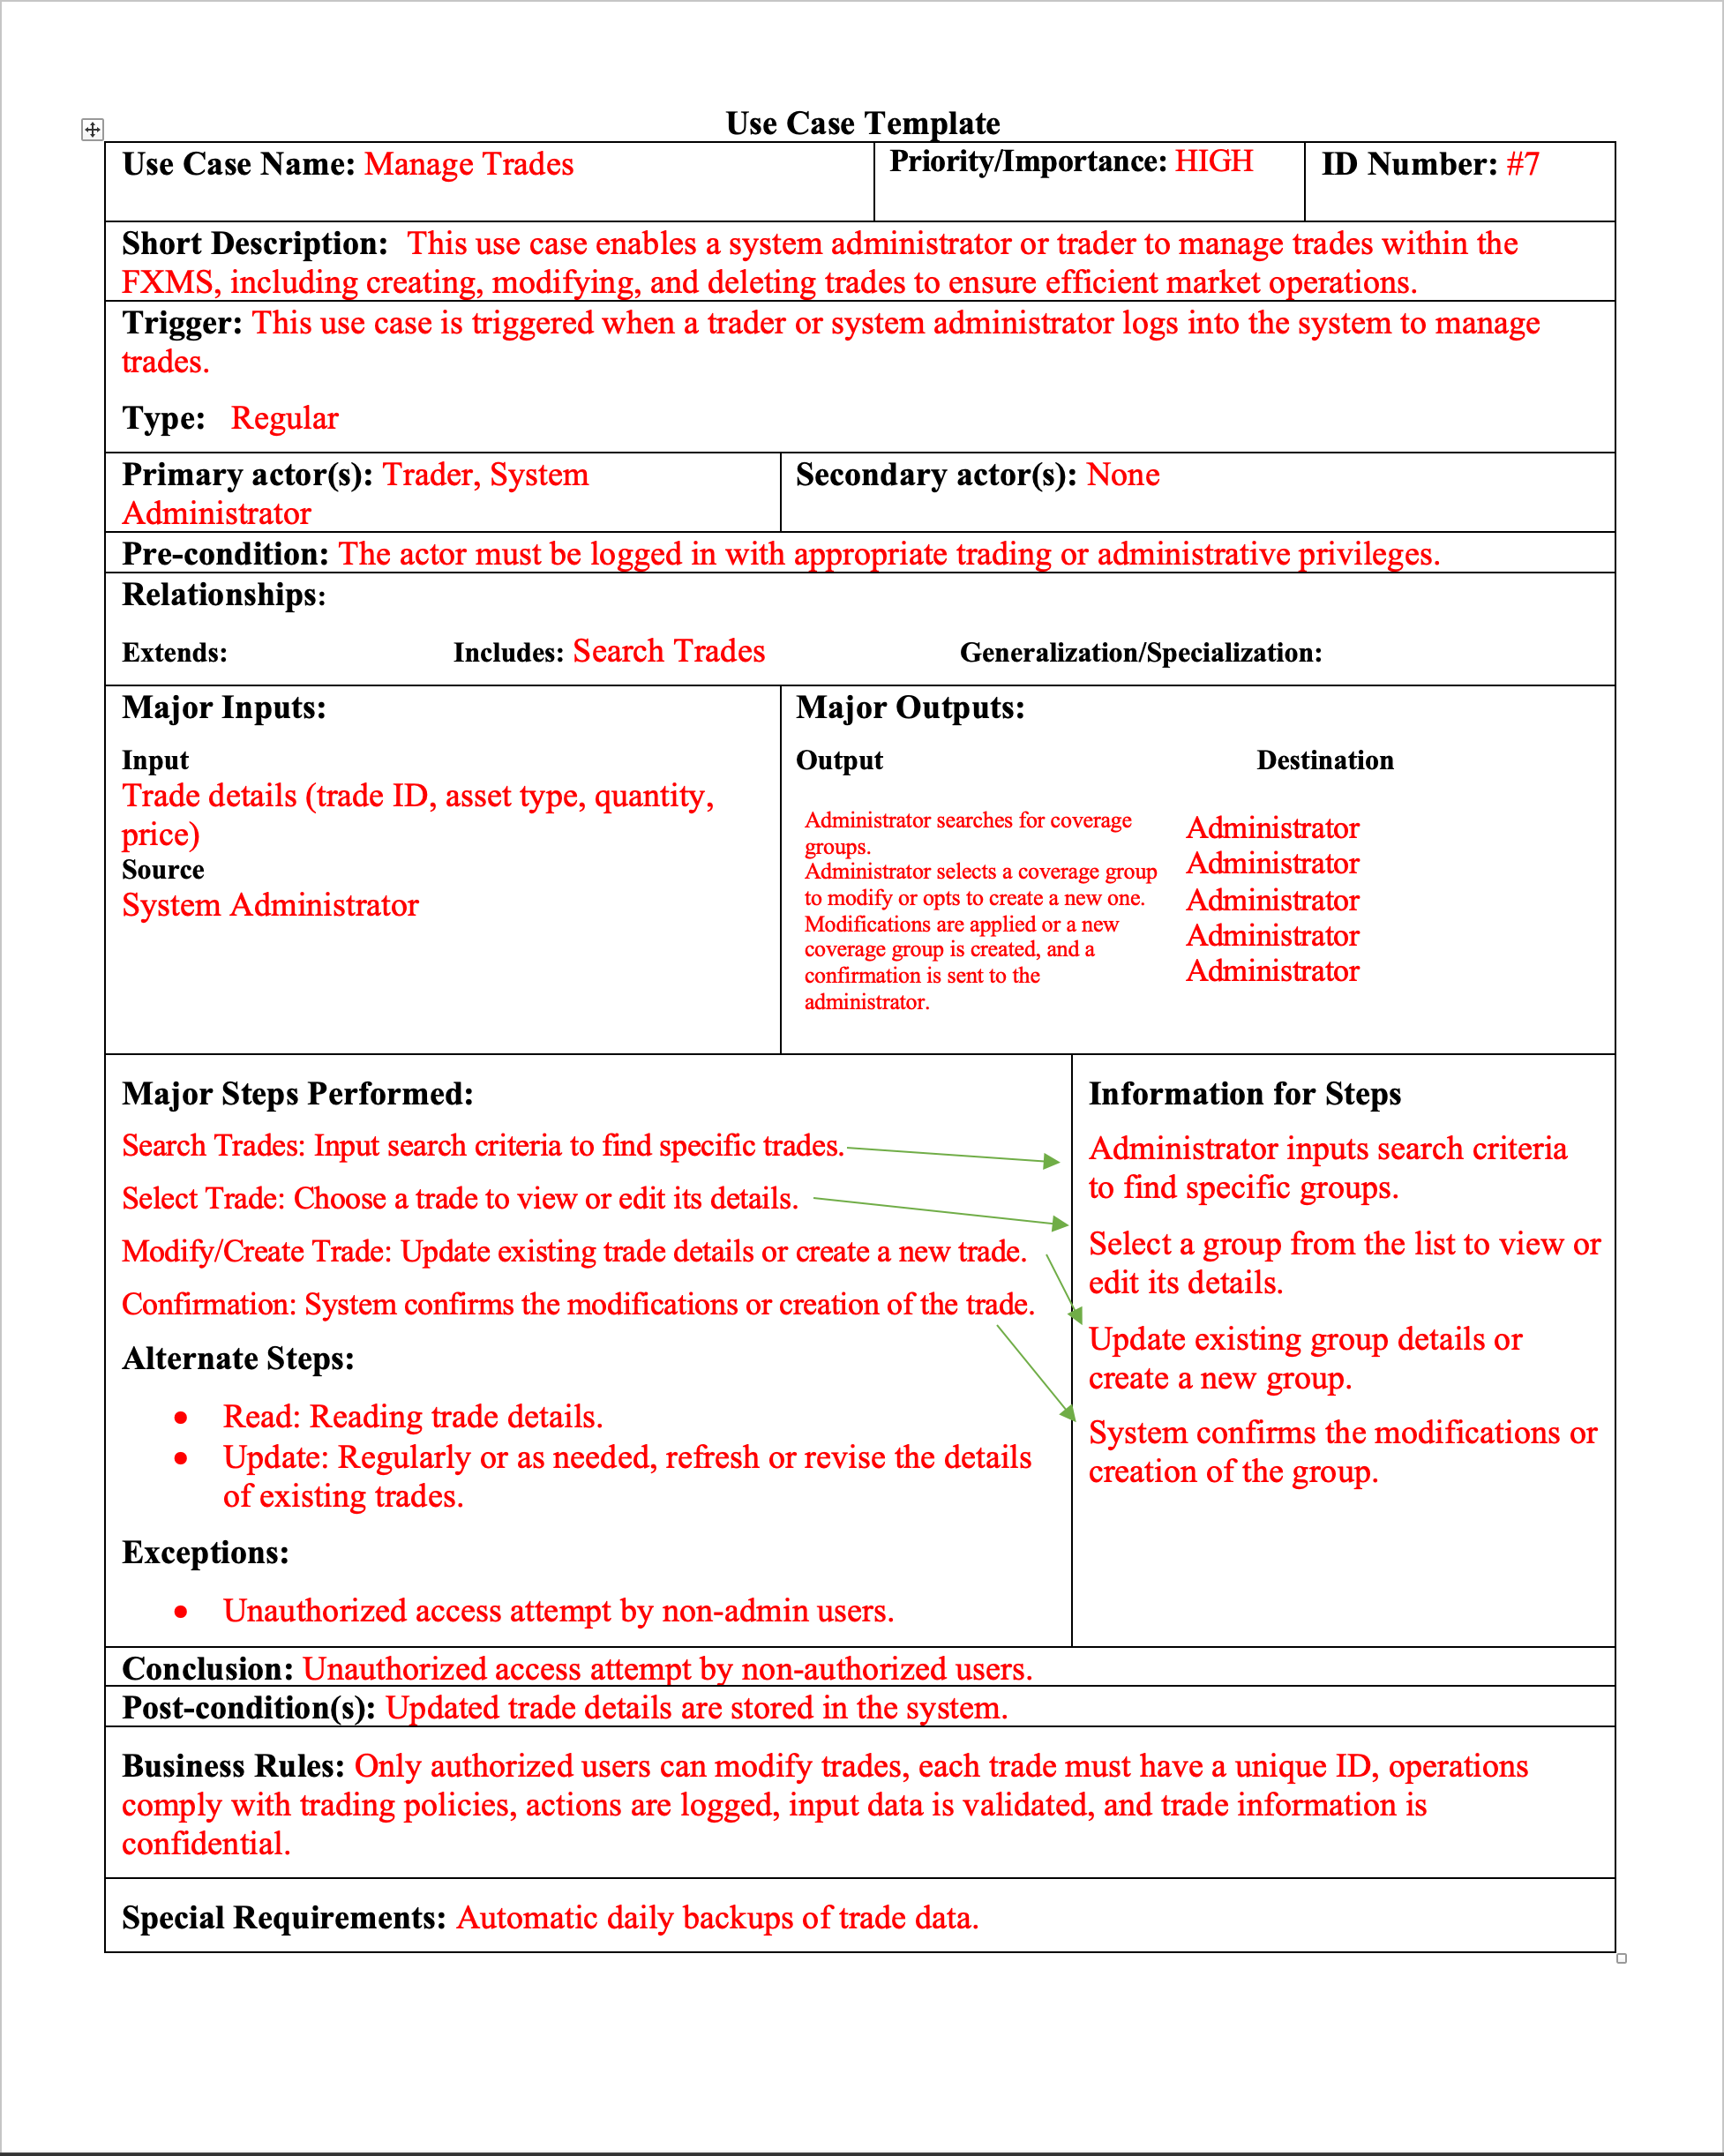
\includegraphics[width=\textwidth]{images/uc/7-manage-trades.png}
    \caption{Manage Trades}
    \label{fig:7-manage-trades}
\end{figure}

\chapter{NFRs Specification}

\begin{enumerate}
    \item \textbf{Usability:} The system shall allow any action for the trader in three or less clicks.
    \item \textbf{Reliability:} The system shall be up 99.99\% of the time.
    \item \textbf{Accuracy:} The system shall save the amounts in integer format using the smallest unit of the currency.
    \item \textbf{Throughput:} The system shall execute 50 trades per second.
    \item \textbf{Security:} The system shall have a role-based access control (RBAC) system.
    \item \textbf{Security:} The system shall have multi-factor mechanism in place.
\end{enumerate}

\end{document}
